%%%%%%%%%%%%%%%%%%%% author.tex %%%%%%%%%%%%%%%%%%%%%%%%%%%%%%%%%%%
%
% sample root file for your "contribution" to a proceedings volume
%
% Use this file as a template for your own input.
%
%%%%%%%%%%%%%%%% Springer %%%%%%%%%%%%%%%%%%%%%%%%%%%%%%%%%%
% to be used for MCQMC 2024
%%%%%%%%%%%%%%%%%%%%%%%%%%%%%%%%%%%%%%%%%%%%%%%%%%%%%%%%%%%%


\documentclass{svproc}
%
% RECOMMENDED %%%%%%%%%%%%%%%%%%%%%%%%%%%%%%%%%%%%%%%%%%%%%%%%%%%
%

% to typeset URLs, URIs, and DOIs
\usepackage{url}
\def\UrlFont{\rmfamily}

%%%%%%%added CL
\usepackage{hyperref}
\usepackage{type1cm}        % activate if the above 3 fonts are
% not available on your system
%
\usepackage{makeidx}         % allows index generation
\usepackage{graphicx}        % standard LaTeX graphics tool
                             % when including figure files
%%% if you are including figures and images, you are encouraged to put them in sub-directory(ies)
%%% whose path(s) can be provided using the following command
%%% \graphicspath{{<path 1>}{<path 2>}}
%%% for example if your sub-directory is called MyFigures then you would use the command
%%% \graphicspath{{MyFigures/}}


\usepackage{multicol}        % used for the two-column index
\usepackage[bottom]{footmisc}% places footnotes at page bottom


\usepackage{newtxtext}       %
\usepackage[varvw]{newtxmath}       % selects Times Roman as basic font

% see the list of further useful packages
% in the Reference Guide

%\makeindex             % used for the subject index
% please use the style svind.ist with
% your makeindex program

%%%%%%%%%%%%%%%%%%%%%%%%%%%%%%%%%%%%%%%%%%%%%%%%%%%%%%%%%%%%%%%%%%%%%%%%%%%%%%%%%%%%%%%%%

% Additional packages
\usepackage{bm}% for bold math symbols
\usepackage{siunitx}% for table alignments

% Additional environment
 \usepackage{mathtools}
% \newtheorem{algorithm}{\upshape Algorithm}[1][]

\newcounter{algorithm}%[section]
\newenvironment{algorithm}[1][]{\refstepcounter{algorithm}\par\medskip
  \noindent\textbf{Algorithm~\thealgorithm\mbox{ }#1}}{\medskip}


%%  This file will be included when we compile the final book. You can
%%  make use of the commonly used packages and commonly defined macros
%%  from here.
%%
%%  PLEASE DO NOT CHANGE THIS FILE.
%%  PLEASE DO NOT REDFINE ANY OF THE MACROS.
%%
%%  For convenience you may wish to define your own macros in your main
%%  tex file while preparing the manuscript. However, before submitting
%%  your final file for the accepted manuscript, we will ask you to replace
%%  your macros with the full commands.
%%

%% OCTOBER 2021 VERSION

% We add the following commonly used macros:

% vectors as boldsymbols:
\newcommand{\bsa}{{\boldsymbol{a}}}
\newcommand{\bsb}{{\boldsymbol{b}}}
\newcommand{\bsc}{{\boldsymbol{c}}}
\newcommand{\bsd}{{\boldsymbol{d}}}
\newcommand{\bse}{{\boldsymbol{e}}}
\newcommand{\bsf}{{\boldsymbol{f}}}
\newcommand{\bsg}{{\boldsymbol{g}}}
\newcommand{\bsh}{{\boldsymbol{h}}}
\newcommand{\bsi}{{\boldsymbol{i}}}
\newcommand{\bsj}{{\boldsymbol{j}}}
\newcommand{\bsk}{{\boldsymbol{k}}}
\newcommand{\bsl}{{\boldsymbol{l}}}
\newcommand{\bsm}{{\boldsymbol{m}}}
\newcommand{\bsn}{{\boldsymbol{n}}}
\newcommand{\bso}{{\boldsymbol{o}}}
\newcommand{\bsp}{{\boldsymbol{p}}}
\newcommand{\bsq}{{\boldsymbol{q}}}
\newcommand{\bsr}{{\boldsymbol{r}}}
\newcommand{\bss}{{\boldsymbol{s}}}
\newcommand{\bst}{{\boldsymbol{t}}}
\newcommand{\bsu}{{\boldsymbol{u}}}
\newcommand{\bsv}{{\boldsymbol{v}}}
\newcommand{\bsw}{{\boldsymbol{w}}}
\newcommand{\bsx}{{\boldsymbol{x}}}
\newcommand{\bsy}{{\boldsymbol{y}}}
\newcommand{\bsz}{{\boldsymbol{z}}}
\newcommand{\bsA}{{\boldsymbol{A}}}
\newcommand{\bsB}{{\boldsymbol{B}}}
\newcommand{\bsC}{{\boldsymbol{C}}}
\newcommand{\bsD}{{\boldsymbol{D}}}
\newcommand{\bsE}{{\boldsymbol{E}}}
\newcommand{\bsF}{{\boldsymbol{F}}}
\newcommand{\bsG}{{\boldsymbol{G}}}
\newcommand{\bsH}{{\boldsymbol{H}}}
\newcommand{\bsI}{{\boldsymbol{I}}}
\newcommand{\bsJ}{{\boldsymbol{J}}}
\newcommand{\bsK}{{\boldsymbol{K}}}
\newcommand{\bsL}{{\boldsymbol{L}}}
\newcommand{\bsM}{{\boldsymbol{M}}}
\newcommand{\bsN}{{\boldsymbol{N}}}
\newcommand{\bsO}{{\boldsymbol{O}}}
\newcommand{\bsP}{{\boldsymbol{P}}}
\newcommand{\bsQ}{{\boldsymbol{Q}}}
\newcommand{\bsR}{{\boldsymbol{R}}}
\newcommand{\bsS}{{\boldsymbol{S}}}
\newcommand{\bsT}{{\boldsymbol{T}}}
\newcommand{\bsU}{{\boldsymbol{U}}}
\newcommand{\bsV}{{\boldsymbol{V}}}
\newcommand{\bsW}{{\boldsymbol{W}}}
\newcommand{\bsX}{{\boldsymbol{X}}}
\newcommand{\bsY}{{\boldsymbol{Y}}}
\newcommand{\bsZ}{{\boldsymbol{Z}}}
% other commonly used boldsymbols:
\newcommand{\bsell}{{\boldsymbol{\ell}}}
\newcommand{\bszero}{{\boldsymbol{0}}} % vector of zeros
\newcommand{\bsone}{{\boldsymbol{1}}}  % vector of ones
% boldsymbol greeks:
\newcommand{\bsalpha}{{\boldsymbol{\alpha}}}
\newcommand{\bsbeta}{{\boldsymbol{\beta}}}
\newcommand{\bsgamma}{{\boldsymbol{\gamma}}}
\newcommand{\bsdelta}{{\boldsymbol{\delta}}}
\newcommand{\bsepsilon}{{\boldsymbol{\epsilon}}}
\newcommand{\bsvarepsilon}{{\boldsymbol{\varepsilon}}}
\newcommand{\bszeta}{{\boldsymbol{\zeta}}}
\newcommand{\bseta}{{\boldsymbol{\eta}}}
\newcommand{\bstheta}{{\boldsymbol{\theta}}}
\newcommand{\bsvartheta}{{\boldsymbol{\vartheta}}}
\newcommand{\bskappa}{{\boldsymbol{\kappa}}}
\newcommand{\bslambda}{{\boldsymbol{\lambda}}}
\newcommand{\bsmu}{{\boldsymbol{\mu}}}
\newcommand{\bsnu}{{\boldsymbol{\nu}}}
\newcommand{\bsxi}{{\boldsymbol{\xi}}}
\newcommand{\bspi}{{\boldsymbol{\pi}}}
\newcommand{\bsvarpi}{{\boldsymbol{\varpi}}}
\newcommand{\bsrho}{{\boldsymbol{\rho}}}
\newcommand{\bsvarrho}{{\boldsymbol{\varrho}}}
\newcommand{\bssigma}{{\boldsymbol{\sigma}}}
\newcommand{\bsvarsigma}{{\boldsymbol{\varsigma}}}
\newcommand{\bstau}{{\boldsymbol{\tau}}}
\newcommand{\bsupsilon}{{\boldsymbol{\upsilon}}}
\newcommand{\bsphi}{{\boldsymbol{\phi}}}
\newcommand{\bsvarphi}{{\boldsymbol{\varphi}}}
\newcommand{\bschi}{{\boldsymbol{\chi}}}
\newcommand{\bspsi}{{\boldsymbol{\psi}}}
\newcommand{\bsomega}{{\boldsymbol{\omega}}}
\newcommand{\bsGamma}{{\boldsymbol{\Gamma}}}
\newcommand{\bsDelta}{{\boldsymbol{\Delta}}}
\newcommand{\bsTheta}{{\boldsymbol{\Theta}}}
\newcommand{\bsLambda}{{\boldsymbol{\Lambda}}}
\newcommand{\bsXi}{{\boldsymbol{\Xi}}}
\newcommand{\bsPi}{{\boldsymbol{\Pi}}}
\newcommand{\bsSigma}{{\boldsymbol{\Sigma}}}
\newcommand{\bsUpsilon}{{\boldsymbol{\Upsilon}}}
\newcommand{\bsPhi}{{\boldsymbol{\Phi}}}
\newcommand{\bsPsi}{{\boldsymbol{\Psi}}}
\newcommand{\bsOmega}{{\boldsymbol{\Omega}}}

% Roman fonts:
\newcommand{\rma}{{\mathrm{a}}}
\newcommand{\rmb}{{\mathrm{b}}}
\newcommand{\rmc}{{\mathrm{c}}}
\newcommand{\rmd}{{\mathrm{d}}}
\newcommand{\rme}{{\mathrm{e}}}
\newcommand{\rmf}{{\mathrm{f}}}
\newcommand{\rmg}{{\mathrm{g}}}
\newcommand{\rmh}{{\mathrm{h}}}
\newcommand{\rmi}{{\mathrm{i}}}
\newcommand{\rmj}{{\mathrm{j}}}
\newcommand{\rmk}{{\mathrm{k}}}
\newcommand{\rml}{{\mathrm{l}}}
\newcommand{\rmm}{{\mathrm{m}}}
\newcommand{\rmn}{{\mathrm{n}}}
\newcommand{\rmo}{{\mathrm{o}}}
\newcommand{\rmp}{{\mathrm{p}}}
\newcommand{\rmq}{{\mathrm{q}}}
\newcommand{\rmr}{{\mathrm{r}}}
\newcommand{\rms}{{\mathrm{s}}}
\newcommand{\rmt}{{\mathrm{t}}}
\newcommand{\rmu}{{\mathrm{u}}}
\newcommand{\rmv}{{\mathrm{v}}}
\newcommand{\rmw}{{\mathrm{w}}}
\newcommand{\rmx}{{\mathrm{x}}}
\newcommand{\rmy}{{\mathrm{y}}}
\newcommand{\rmz}{{\mathrm{z}}}
\newcommand{\rmA}{{\mathrm{A}}}
\newcommand{\rmB}{{\mathrm{B}}}
\newcommand{\rmC}{{\mathrm{C}}}
\newcommand{\rmD}{{\mathrm{D}}}
\newcommand{\rmE}{{\mathrm{E}}}
\newcommand{\rmF}{{\mathrm{F}}}
\newcommand{\rmG}{{\mathrm{G}}}
\newcommand{\rmH}{{\mathrm{H}}}
\newcommand{\rmI}{{\mathrm{I}}}
\newcommand{\rmJ}{{\mathrm{J}}}
\newcommand{\rmK}{{\mathrm{K}}}
\newcommand{\rmL}{{\mathrm{L}}}
\newcommand{\rmM}{{\mathrm{M}}}
\newcommand{\rmN}{{\mathrm{N}}}
\newcommand{\rmO}{{\mathrm{O}}}
\newcommand{\rmP}{{\mathrm{P}}}
\newcommand{\rmQ}{{\mathrm{Q}}}
\newcommand{\rmR}{{\mathrm{R}}}
\newcommand{\rmS}{{\mathrm{S}}}
\newcommand{\rmT}{{\mathrm{T}}}
\newcommand{\rmU}{{\mathrm{U}}}
\newcommand{\rmV}{{\mathrm{V}}}
\newcommand{\rmW}{{\mathrm{W}}}
\newcommand{\rmX}{{\mathrm{X}}}
\newcommand{\rmY}{{\mathrm{Y}}}
\newcommand{\rmZ}{{\mathrm{Z}}}
% also commonly defined
\newcommand{\rd}{{\mathrm{d}}}
\newcommand{\ri}{{\mathrm{i}}}

% blackboards:
\newcommand{\bbA}{{\mathbb{A}}}
\newcommand{\bbB}{{\mathbb{B}}}
\newcommand{\bbC}{{\mathbb{C}}}
\newcommand{\bbD}{{\mathbb{D}}}
\newcommand{\bbE}{{\mathbb{E}}}
\newcommand{\bbF}{{\mathbb{F}}}
\newcommand{\bbG}{{\mathbb{G}}}
\newcommand{\bbH}{{\mathbb{H}}}
\newcommand{\bbI}{{\mathbb{I}}}
\newcommand{\bbJ}{{\mathbb{J}}}
\newcommand{\bbK}{{\mathbb{K}}}
\newcommand{\bbL}{{\mathbb{L}}}
\newcommand{\bbM}{{\mathbb{M}}}
\newcommand{\bbN}{{\mathbb{N}}}
\newcommand{\bbO}{{\mathbb{O}}}
\newcommand{\bbP}{{\mathbb{P}}}
\newcommand{\bbQ}{{\mathbb{Q}}}
\newcommand{\bbR}{{\mathbb{R}}}
\newcommand{\bbS}{{\mathbb{S}}}
\newcommand{\bbT}{{\mathbb{T}}}
\newcommand{\bbU}{{\mathbb{U}}}
\newcommand{\bbV}{{\mathbb{V}}}
\newcommand{\bbW}{{\mathbb{W}}}
\newcommand{\bbX}{{\mathbb{X}}}
\newcommand{\bbY}{{\mathbb{Y}}}
\newcommand{\bbZ}{{\mathbb{Z}}}
% commonly used shortcuts:
\newcommand{\C}{{\mathbb{C}}} % complex numbers
\newcommand{\F}{{\mathbb{F}}} % field, finite field
\newcommand{\N}{{\mathbb{N}}} % natural numbers {1, 2, ...}
\newcommand{\Q}{{\mathbb{Q}}} % rationals
\newcommand{\R}{{\mathbb{R}}} % reals
\newcommand{\Z}{{\mathbb{Z}}} % integers
% more commonly used shortcuts:
\newcommand{\CC}{{\mathbb{C}}} % complex numbers
\newcommand{\FF}{{\mathbb{F}}} % field, finite field
\newcommand{\NN}{{\mathbb{N}}} % natural numbers {1, 2, ...}
\newcommand{\QQ}{{\mathbb{Q}}} % rationals
\newcommand{\RR}{{\mathbb{R}}} % reals
\newcommand{\ZZ}{{\mathbb{Z}}} % integers
% more commonly used shortcuts:
\newcommand{\EE}{{\mathbb{E}}}
\newcommand{\PP}{{\mathbb{P}}}
\newcommand{\TT}{{\mathbb{T}}}
\newcommand{\VV}{{\mathbb{V}}}
% and even more commonly used shortcuts:
\newcommand{\Complex}{{\mathbb{C}}}
\newcommand{\Integer}{{\mathbb{Z}}}
\newcommand{\Natural}{{\mathbb{N}}}
\newcommand{\Rational}{{\mathbb{Q}}}
\newcommand{\Real}{{\mathbb{R}}}
% indicator boldface 1:
\DeclareSymbolFont{bbold}{U}{bbold}{m}{n}
\DeclareSymbolFontAlphabet{\mathbbold}{bbold}
\newcommand{\ind}{{\mathbbold{1}}}
\newcommand{\bbone}{{\mathbbold{1}}}


% calligraphic letters:
\newcommand{\cala}{{\mathcal{a}}}
\newcommand{\calb}{{\mathcal{b}}}
\newcommand{\calc}{{\mathcal{c}}}
\newcommand{\cald}{{\mathcal{d}}}
\newcommand{\cale}{{\mathcal{e}}}
\newcommand{\calf}{{\mathcal{f}}}
\newcommand{\calg}{{\mathcal{g}}}
\newcommand{\calh}{{\mathcal{h}}}
\newcommand{\cali}{{\mathcal{i}}}
\newcommand{\calj}{{\mathcal{j}}}
\newcommand{\calk}{{\mathcal{k}}}
\newcommand{\call}{{\mathcal{l}}}
\newcommand{\calm}{{\mathcal{m}}}
\newcommand{\caln}{{\mathcal{n}}}
\newcommand{\calo}{{\mathcal{o}}}
\newcommand{\calp}{{\mathcal{p}}}
\newcommand{\calq}{{\mathcal{q}}}
\newcommand{\calr}{{\mathcal{r}}}
\newcommand{\cals}{{\mathcal{s}}}
\newcommand{\calt}{{\mathcal{t}}}
\newcommand{\calu}{{\mathcal{u}}}
\newcommand{\calv}{{\mathcal{v}}}
\newcommand{\calw}{{\mathcal{w}}}
\newcommand{\calx}{{\mathcal{x}}}
\newcommand{\caly}{{\mathcal{y}}}
\newcommand{\calz}{{\mathcal{z}}}
\newcommand{\calA}{{\mathcal{A}}}
\newcommand{\calB}{{\mathcal{B}}}
\newcommand{\calC}{{\mathcal{C}}}
\newcommand{\calD}{{\mathcal{D}}}
\newcommand{\calE}{{\mathcal{E}}}
\newcommand{\calF}{{\mathcal{F}}}
\newcommand{\calG}{{\mathcal{G}}}
\newcommand{\calH}{{\mathcal{H}}}
\newcommand{\calI}{{\mathcal{I}}}
\newcommand{\calJ}{{\mathcal{J}}}
\newcommand{\calK}{{\mathcal{K}}}
\newcommand{\calL}{{\mathcal{L}}}
\newcommand{\calM}{{\mathcal{M}}}
\newcommand{\calN}{{\mathcal{N}}}
\newcommand{\calO}{{\mathcal{O}}}
\newcommand{\calP}{{\mathcal{P}}}
\newcommand{\calQ}{{\mathcal{Q}}}
\newcommand{\calR}{{\mathcal{R}}}
\newcommand{\calS}{{\mathcal{S}}}
\newcommand{\calT}{{\mathcal{T}}}
\newcommand{\calU}{{\mathcal{U}}}
\newcommand{\calV}{{\mathcal{V}}}
\newcommand{\calW}{{\mathcal{W}}}
\newcommand{\calX}{{\mathcal{X}}}
\newcommand{\calY}{{\mathcal{Y}}}
\newcommand{\calZ}{{\mathcal{Z}}}

% Euler fraks:
\newcommand{\fraka}{{\mathfrak{a}}}
\newcommand{\frakb}{{\mathfrak{b}}}
\newcommand{\frakc}{{\mathfrak{c}}}
\newcommand{\frakd}{{\mathfrak{d}}}
\newcommand{\frake}{{\mathfrak{e}}}
\newcommand{\frakf}{{\mathfrak{f}}}
\newcommand{\frakg}{{\mathfrak{g}}}
\newcommand{\frakh}{{\mathfrak{h}}}
\newcommand{\fraki}{{\mathfrak{i}}}
\newcommand{\frakj}{{\mathfrak{j}}}
\newcommand{\frakk}{{\mathfrak{k}}}
\newcommand{\frakl}{{\mathfrak{l}}}
\newcommand{\frakm}{{\mathfrak{m}}}
\newcommand{\frakn}{{\mathfrak{n}}}
\newcommand{\frako}{{\mathfrak{o}}}
\newcommand{\frakp}{{\mathfrak{p}}}
\newcommand{\frakq}{{\mathfrak{q}}}
\newcommand{\frakr}{{\mathfrak{r}}}
\newcommand{\fraks}{{\mathfrak{s}}}
\newcommand{\frakt}{{\mathfrak{t}}}
\newcommand{\fraku}{{\mathfrak{u}}}
\newcommand{\frakv}{{\mathfrak{v}}}
\newcommand{\frakw}{{\mathfrak{w}}}
\newcommand{\frakx}{{\mathfrak{x}}}
\newcommand{\fraky}{{\mathfrak{y}}}
\newcommand{\frakz}{{\mathfrak{z}}}
\newcommand{\frakA}{{\mathfrak{A}}}
\newcommand{\frakB}{{\mathfrak{B}}}
\newcommand{\frakC}{{\mathfrak{C}}}
\newcommand{\frakD}{{\mathfrak{D}}}
\newcommand{\frakE}{{\mathfrak{E}}}
\newcommand{\frakF}{{\mathfrak{F}}}
\newcommand{\frakG}{{\mathfrak{G}}}
\newcommand{\frakH}{{\mathfrak{H}}}
\newcommand{\frakI}{{\mathfrak{I}}}
\newcommand{\frakJ}{{\mathfrak{J}}}
\newcommand{\frakK}{{\mathfrak{K}}}
\newcommand{\frakL}{{\mathfrak{L}}}
\newcommand{\frakM}{{\mathfrak{M}}}
\newcommand{\frakN}{{\mathfrak{N}}}
\newcommand{\frakO}{{\mathfrak{O}}}
\newcommand{\frakP}{{\mathfrak{P}}}
\newcommand{\frakQ}{{\mathfrak{Q}}}
\newcommand{\frakR}{{\mathfrak{R}}}
\newcommand{\frakS}{{\mathfrak{S}}}
\newcommand{\frakT}{{\mathfrak{T}}}
\newcommand{\frakU}{{\mathfrak{U}}}
\newcommand{\frakV}{{\mathfrak{V}}}
\newcommand{\frakW}{{\mathfrak{W}}}
\newcommand{\frakX}{{\mathfrak{X}}}
\newcommand{\frakY}{{\mathfrak{Y}}}
\newcommand{\frakZ}{{\mathfrak{Z}}}
% sets as Euler fraks:
\newcommand{\seta}{{\mathfrak{a}}}
\newcommand{\setb}{{\mathfrak{b}}}
\newcommand{\setc}{{\mathfrak{c}}}
\newcommand{\setd}{{\mathfrak{d}}}
\newcommand{\sete}{{\mathfrak{e}}}
\newcommand{\setf}{{\mathfrak{f}}}
\newcommand{\setg}{{\mathfrak{g}}}
\newcommand{\seth}{{\mathfrak{h}}}
\newcommand{\seti}{{\mathfrak{i}}}
\newcommand{\setj}{{\mathfrak{j}}}
\newcommand{\setk}{{\mathfrak{k}}}
\newcommand{\setl}{{\mathfrak{l}}}
\newcommand{\setm}{{\mathfrak{m}}}
\newcommand{\setn}{{\mathfrak{n}}}
\newcommand{\seto}{{\mathfrak{o}}}
\newcommand{\setp}{{\mathfrak{p}}}
\newcommand{\setq}{{\mathfrak{q}}}
\newcommand{\setr}{{\mathfrak{r}}}
\newcommand{\sets}{{\mathfrak{s}}}
\newcommand{\sett}{{\mathfrak{t}}}
\newcommand{\setu}{{\mathfrak{u}}}
\newcommand{\setv}{{\mathfrak{v}}}
\newcommand{\setw}{{\mathfrak{w}}}
\newcommand{\setx}{{\mathfrak{x}}}
\newcommand{\sety}{{\mathfrak{y}}}
\newcommand{\setz}{{\mathfrak{z}}}
\newcommand{\setA}{{\mathfrak{A}}}
\newcommand{\setB}{{\mathfrak{B}}}
\newcommand{\setC}{{\mathfrak{C}}}
\newcommand{\setD}{{\mathfrak{D}}}
\newcommand{\setE}{{\mathfrak{E}}}
\newcommand{\setF}{{\mathfrak{F}}}
\newcommand{\setG}{{\mathfrak{G}}}
\newcommand{\setH}{{\mathfrak{H}}}
\newcommand{\setI}{{\mathfrak{I}}}
\newcommand{\setJ}{{\mathfrak{J}}}
\newcommand{\setK}{{\mathfrak{K}}}
\newcommand{\setL}{{\mathfrak{L}}}
\newcommand{\setM}{{\mathfrak{M}}}
\newcommand{\setN}{{\mathfrak{N}}}
\newcommand{\setO}{{\mathfrak{O}}}
\newcommand{\setP}{{\mathfrak{P}}}
\newcommand{\setQ}{{\mathfrak{Q}}}
\newcommand{\setR}{{\mathfrak{R}}}
\newcommand{\setS}{{\mathfrak{S}}}
\newcommand{\setT}{{\mathfrak{T}}}
\newcommand{\setU}{{\mathfrak{U}}}
\newcommand{\setV}{{\mathfrak{V}}}
\newcommand{\setW}{{\mathfrak{W}}}
\newcommand{\setX}{{\mathfrak{X}}}
\newcommand{\setY}{{\mathfrak{Y}}}
\newcommand{\setZ}{{\mathfrak{Z}}}

% other commonly defined commands:
\newcommand{\wal}{{\rm wal}}
\newcommand{\floor}[1]{\left\lfloor #1 \right\rfloor} % floor
\newcommand{\ceil}[1]{\left\lceil #1 \right\rceil}    % ceil
\DeclareMathOperator{\cov}{Cov}
\DeclareMathOperator{\var}{Var}
\providecommand{\argmin}{\operatorname*{argmin}}
\providecommand{\argmax}{\operatorname*{argmax}}
%%%% end added CL


%%Fred's temporary macros
\newcommand{\figpath}{Figures}
\usepackage{xspace}

%%End of Fred's temporary macros


\begin{document}


\mainmatter              % start of a contribution
%
\title{Quasi-Monte Carlo Methods:  What, Why, and How?}
%
\titlerunning{Quasi-Monte Carlo Methods}  % abbreviated title (for running head)
%                                     also used for the TOC unless
%                                     \toctitle is used
%
\author{Fred J. Hickernell\inst{1} \and Nathan Kirk\inst{2} \and Aleksei G. Sorokin\inst{3}}
%
\authorrunning{Hickernell, Kirk, and Sorokin} % abbreviated author list (for running head)
%
%%%% list of authors for the TOC (use if author list has to be modified)
\tocauthor{Fred J. Hickernell, Nathan Kirk, Aleksei G. Sorokin}
%
\institute{
Department of Applied Mathematics, Illinois Institute of Technology, \\ Chicago, IL, 60616, USA\\
\email{hickernell@iit.edu}, \
\texttt{http://www.iit.edu/~hickernell}
\and
\email{nkirk@iit.edu}
\and
\email{asorokin@hawk.iit.edu}
}



\maketitle              % typeset the title of the contribution

\begin{abstract}
Many problems in  quantitative finance, uncertainty quantification, and other disiplines are answered by computing the population mean, $\mu := \mathbb{E}(Y)$, where instances of $Y:=f(\boldsymbol{X})$ may be generated by numerical simulation and $\bsX$ has a simple probability  distribution. The population mean can be approximated by the sample mean, $\hat{\mu}_n := n^{-1} \sum_{i=0}^{n-1} f(\bsx_i)$ for a well chosen sequence of nodes, $\{\bsx_0, \bsx_1, \ldots\}$ and a sufficiently large sample size, $n$.  Computing $\mu$ is equivalent to computing a $d$-dimensional integral, $\int f(\bsx) \varrho(\bsx) \, \mathrm{d} \bsx$, where $\varrho$ is the probability density for $\bsX$.

Quasi-Monte Carlo methods replace independent and identically distributed  sequences of random vector nodes, $\{\bsx_i \}_{i = 0}^{\infty}$, by low discrepancy sequences.  This accelerates the convergence of $\hat{\mu}_n$ to $\mu$ as $n \to \infty$.

This tutorial describes  low discrepancy sequences  and their quality measures.  We demonstrate the performance gains possible with quasi-Monte Carlo methods.  Moreover, we describe how to formulate problems to realize the greatest performance gains using quasi-Monte Carlo methods.  We also briefly describe the use of quasi-Monte Carlo methods for problems beyond computing the mean, $\mu$.

\keywords{}
\end{abstract}
%
\setcounter{tocdepth}{2}
\tableofcontents

\section{Introduction} \label{sec:intro}
There are may settings where key underlying quantities that affect the outcome are unknown, e.g.,
\begin{itemize}
	\item Future market forces, which affect financial risk,
	\item The porosity of rock, which affects the extraction of oil or gas, or
	\item Elemetary particle interactions in a high energy physics experiment, which affect what is observed by detectors.
\end{itemize}
In such situations, the unknown inputs are often modeled using random vector variables or stochastic processes.  Computations are performed by generating a multidude of possible outcomes informed by the assumed probability distribution of the input. These are used to estimate the mean, quantiles, and/or probability distribution of the outcome.  This is the essence of the Monte Carlo (MC) method.

In mathematical terms, the random outcome is $Y := f(\bsX)$, where $\bsX$ is a vector random input.  Given a particular input value, $\bsx$, the corresponding outcome  $y = f(\bsx)$ can be computed by an algorithm, whose complexity may be such that $f$ can be considered a ``black box''.  The user selects a sequence of input values, also known as data sites or \emph{nodes}, $\bsx_0, \bsx_1, \ldots$, which give rise to the observed outcomes $y_0 = f(\bsx_0), y_1 = f(\bsx_1), \ldots$.  The $y_i$ form the basis for approximating $\bbE(Y)$, quartiles of $Y$, the probability density of $Y$, and other quantities of interest.

Simple  Monte Carlo chooses the nodes $\{\bsx_0, \bsx_1, \ldots\}$ to be independent and identically distributed (IID).  Quasi-Monte Carlo (qMC)  chooses the nodes \emph{not} IID, but with an empirical distribution that approximates well the true probability distribution of $\bsX$.  The difference between these two distributions is called a \emph{discrepancy}, and the node sequences used in qMC are called low discrepancy (LD) sequences.

This tutorial describes what qMC is, why we would want to use qMC, and how qMC can be implemented well.  The next session illustrates by example the advantages of qMC.  This is followed by a description of how deterministic LD sequences are constructed and randomizations that preserve their low discrepancy.  We describe various measures of discrepancy.  We explain how to decide what sample size, $n$, is sufficient to meet the user's error criterion.  We then discuss how to rewrite the problem of interest in a qMC-friendly way.


%
\section{An Illustration of Quasi-Monte Carlo} \label{sec:practice}

We illustrate the benefits of qMC with an example from Keister \cite{Kei96}, motivated by computational physics:

\begin{equation}\label{eq:keisterA}
	\mu := \int_{\mathbb{R}^d} \cos(\lVert \bst \rVert) \exp(-\lVert \bst \rVert^2) \, \rmd \bst,
\end{equation}
where $\lVert \bst \rVert := \sqrt{t_1^2 + \cdots + t_d^2}$.  This integral may be evaluated numerically by re-writing it in spherical coordinates as
\begin{equation}\label{eq:keisterExact}
	\mu = \frac{2 \pi^{d/2}}{\Gamma(d/2)}\int_{0}^{\infty} \cos(r) \exp(-r^2) \, r^{d-1} \rmd r,
\end{equation}
where $2 \pi^{d/2}/\Gamma(d/2)$ is the surface area of the sphere in $d$ dimensions, and $\Gamma$ is the Gamma function.  The resulting one-dimensional integral is amenable to quadrature methods \cite{}.  This non-trivial test case with a true value that can be easily calculated allows us to compute the numerical errors of various cubature schemes.

However, for the purpose of this illustration, we work with $\mu$ in its original form, \eqref{eq:keisterA} and approximate it by a sample mean,
\begin{equation} \label{eq:sample_mean}
	\hat{\mu}_n := \frac 1n \sum_{i=1}^n f(\bsx_i).
\end{equation}
This does require some further preparation, which is discussed in greater generality in Section \ref{sec:reformulate}.

This $\mu$ may be thought of as the expectation of $Y := g(\bsT) := \pi^{d/2} \cos(\lVert \bsT \rVert)$, where $T_1, \ldots, T_d$ are IID Gaussian (normal) random variables with zero mean and variance $1/2$, i.e., $\bsT :=(T_1, \ldots, T_d) \sim \calN(\bszero,\mathsf{I}/2)$:
\begin{equation}\label{eq:keisterB}
	\mu = \int_{\mathbb{R}^d} \underbrace{\pi^{d/2} \cos(\lVert \bst \rVert)}_{=:g(\bst)} \cdot \underbrace{\frac{\exp(-\lVert \bst \rVert^2)}{\pi^{d/2}}}_{\text{density of } \calN(\bszero,\mathsf{I}/2)} \, \rmd \bst = \bbE(Y) = \bbE[g(\bsT)].
\end{equation}
Nearly all LD sequences, which underlie qMC, are defined to approximate the standard uniform distribution, $\calU[0,1]^d$.  Thus, we perform a variable transformation $\bst = \bigl (\Phi^{-1}(x_1), \ldots, \Phi^{-1}(x_d) \bigr )/\sqrt{2}$,
where is $\Phi$ is the cumulative distribution function of the standard Gaussian random variable.  This reimagines the integral $\mu$ as the expectation of a function, $f$, of a standard uniform random variable:
\begin{multline}\label{eq:keisterC}
	\mu = \int_{[0,1]^d} \underbrace{\pi^{d/2} \cos\Bigl (\bigl \lVert \bigl( \Phi^{-1}(x_1), \ldots, \Phi^{-1}(x_d)\bigr) \bigr\rVert/\sqrt{2}  \Bigr)}_{=:f(\bsx)} \, \rmd \bsx \\
	= \bbE[Y]
	= \bbE[f(\bsX)], \qquad \bsX \sim \calU[0,1]^d.
\end{multline}

Now we can apply IID MC, qMC, and other computational methods to approximate $\mu$ by the sample mean
\begin{equation} \label{eq:sample_mean_Keister}
	\hat{\mu}_n = \frac 1n \sum_{i=1}^n \pi^{d/2} \cos\Bigl (\bigl \lVert \bigl( \Phi^{-1}(x_{i1}), \ldots, \Phi^{-1}(x_{id})\bigr) \bigr\rVert/\sqrt{2}  \Bigr).
\end{equation}
Consider the specific case of $d=6$ for which $\mu \approx -2.327303729298$.  We approximate $\mu$ by the sample mean defined in \eqref{eq:sample_mean} for three different kinds of nodes, $\{\bsx_i\}_{i=0}^{n-1}$, for various sample sizes, $n$, and plot the relative errors, $\lvert (\mu - 	\hat{\mu}_n)/\mu\rvert$ in Figure \ref{fig:keister-err}. The three kind of nodes are
\begin{enumerate}
	\renewcommand{\labelenumi}{\roman{enumi}.}
	\item Cartesian grids, $\{1/(2m), \ldots, (2m-1)/(2m) \}^6$, for $m = 2, 3, \ldots$ and $n = m^6$ (blue),
	\item IID sequences with arbitrary $n$ (orange), and
	\item Randomized LD (Sobol') sequences with $n = 1, 2, \ldots, 2^m, \ldots $ (green).
\end{enumerate}

\begin{figure}
	\centering
	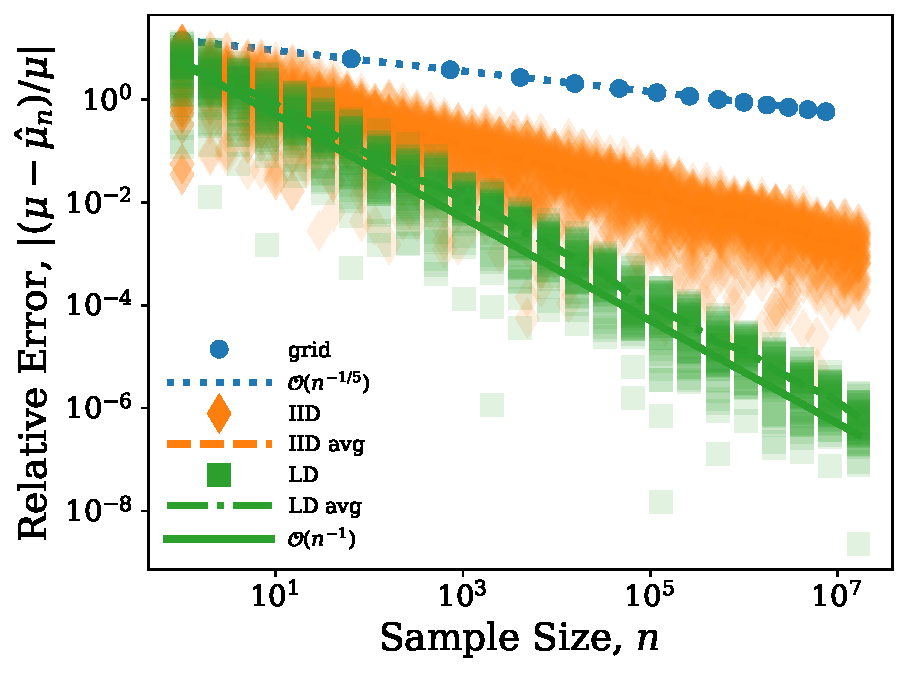
\includegraphics[width =10cm]{\figpath/n_is_16777216_d_is_6_n_rep_is_50_KeisterErrors.pdf}
	\caption{The relative error of approximating $\mu$ defined in \eqref{eq:keisterC} by the sample mean, $\hat{\mu}_n$, defined in \eqref{eq:sample_mean} for various choices of nodes, $\bsx_0, \bsx_1, \ldots$.  Grids have the largest error and LD nodes have the smallest error. \label{fig:keister-err}}
\end{figure}

Note the following from this example:
\begin{itemize}
	\item This integral is not particularly easy to evaluate numerically.  Even the best choice of nodes requires at least $n=100$ to get a relative error below $10\%$.

	\item \emph{Grid nodes.} Although grids may be attractive for low dimensional problems, e.g., $d = 1$, $2$, or $3$, they do poorly for this modest dimension, $d=6$.  Figure \ref{fig:grid} compares a $64$ point grid with $d = 2$ and $6$.  For $d = 6$, the possible sample sizes, $n$, are quite sparse, as shown in Figure \ref{fig:keister-err}.

	Choosing the nodes to lie on a grid corresponds to a tensor product midpoint cubature rule, which would normally be expected to have an error of $\mathcal{O}(n^{-2/d})$  for general $d$.  The error decay of $\mathcal{O}(n^{-1/5})$ rather than $\mathcal{O}(n^{-2/6})$ for this example may be due to the lack of smoothness of $f$ near the boundaries of the unit cube.

	\item \emph{IID nodes.}  Simple MC (orange) is a substantial improvement over grid nodes. As a reminder, for IID nodes the root mean squared error is
	\begin{equation}\label{eq:IIDerror}
		\sqrt{\mathbb{E}[(\mu - \hat{\mu})^2]} = \sqrt{\var(\hat{\mu})} = \sqrt{\frac{\var(f(\bsX))}{n}} = \frac{\mathrm{Std}(f(\bsX))}{n^{1/2}},
	\end{equation}
	where $\var$ denotes the variance and $\mathrm{Std}$ the standard deviation.  This $\mathcal{O}(n^{-1/2})$ decay is observed in Figure \ref{fig:keister-err}. For simple MC the sample size, $n$, can be any positive integer without affecting the rate of decay of the error.

	Whereas grid points collapse on top of one another when viewed in low dimensional projections (Figure \ref{fig:grid}), all IID points may be seen when viewed in any lower dimensional projection, as seen in Figure \ref{fig:iid}.  The disadvantage of IID points is that they form clusters and leave gaps.  This is because the position of any one node is independent of the position of the others.

	\item \emph{LD nodes.}  For qMC methods the error decays nearly like $\mathcal{O}(n^{-1})$, which for this example correponds to a reduction in error of several orders of magnitude compared to simple MC for large enough $n$.  Typically, LD sequences have preferred sample sizes.  For this Sobol' sequence, $n$ is chosen to be non-negative integer powers of $2$, which tends to give better accuracy than arbitrary $n$.

	Figure \ref{fig:ld} shows typical two-dimensional projections of a size $64$ LD node set.  Visually, these nodes fill the unit cube better than IID nodes.  A quantitative measure of this, the discrepancy, is defined in Section \ref{sec:discrepancy}.  Constructions of LD node sequences are explained in the next section.

\end{itemize}

\begin{figure}
	\centering
	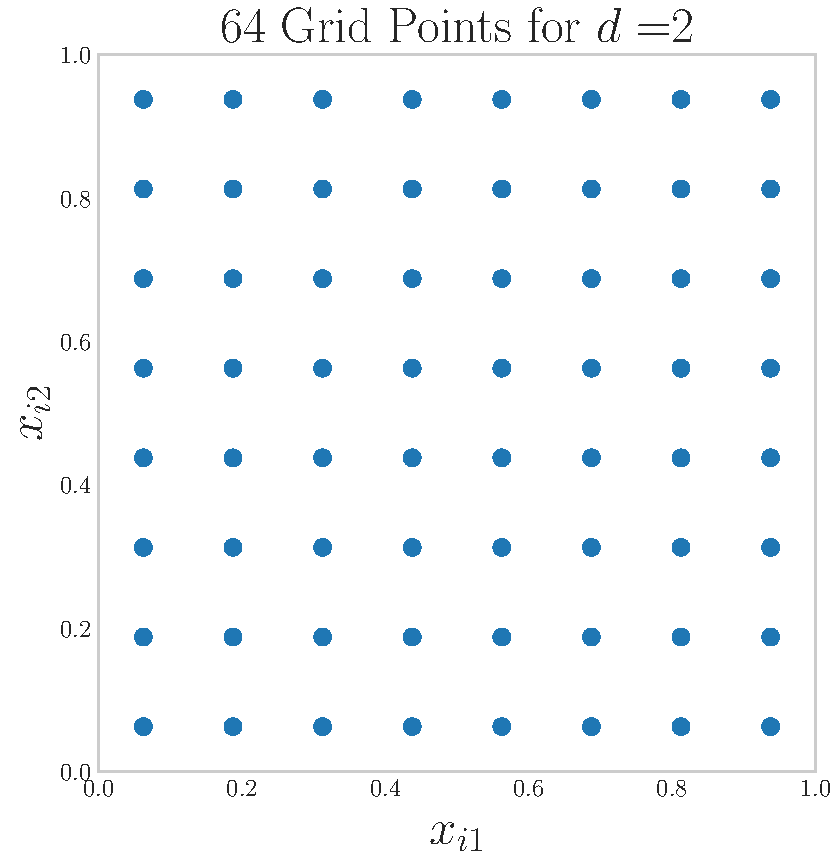
\includegraphics[width = 0.48\textwidth]{\figpath/64gridpts_d2.pdf}\quad
	%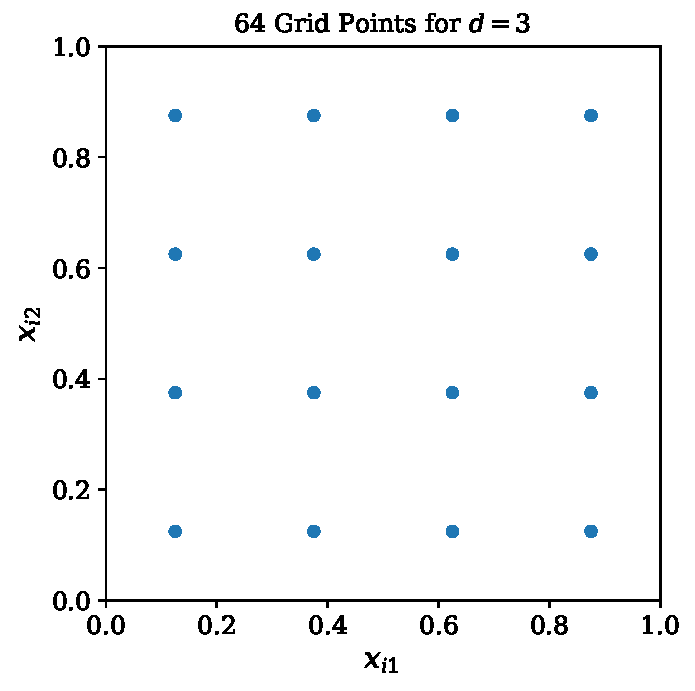
\includegraphics[width = 5cm]{\figpath/64gridpts_d3.pdf}\quad
	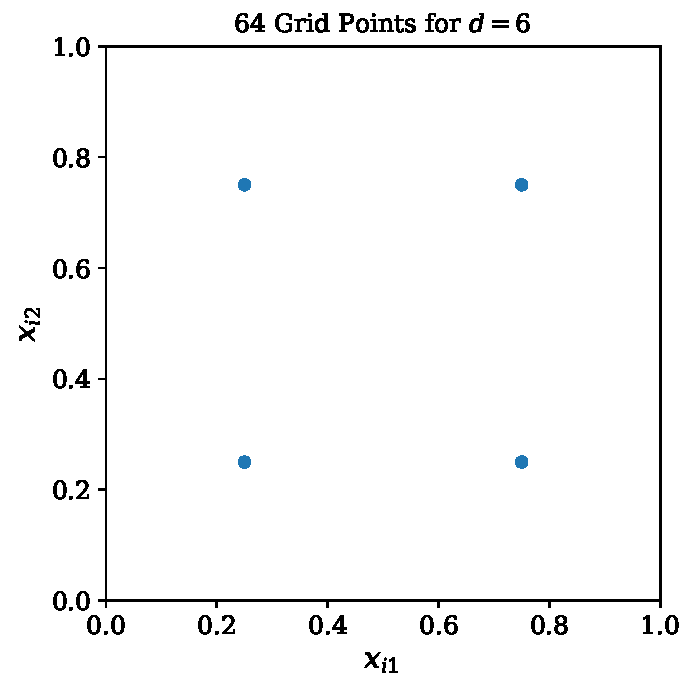
\includegraphics[width =  0.48\textwidth]{\figpath/64gridpts_d6.pdf}
	\caption{Although a two-dimensional grid covers the unit square rather well, a $d$-dimensional grid for modest $d$ does \emph{not} cover the unit cube well.  For example, one can only see four distinct points in a two dimensional projection of a six-dimensional grid with $64$ points. \label{fig:grid}}
\end{figure}

\begin{figure}
	\centering
	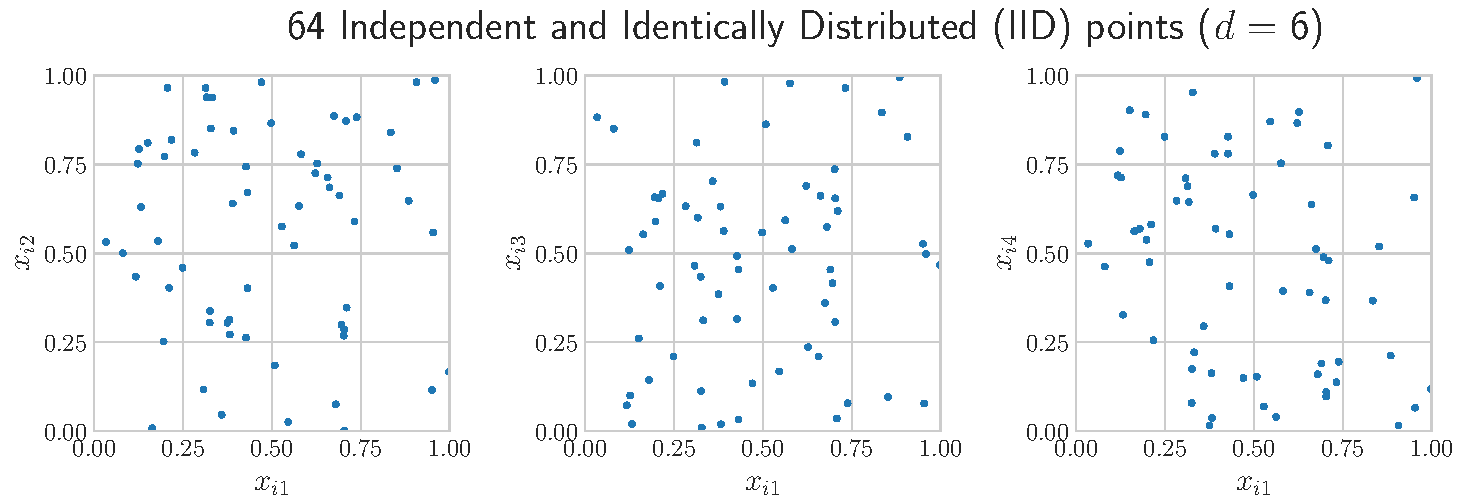
\includegraphics[width =\textwidth]{\figpath/64iidpts_d6.pdf}
	\caption{IID points cover the unit cube better than grid points, although one does observe clusters and gaps.  In any  projection there is  a similar looking distribution of all $64$ points \label{fig:iid}}
\end{figure}

\begin{figure}
	\centering
	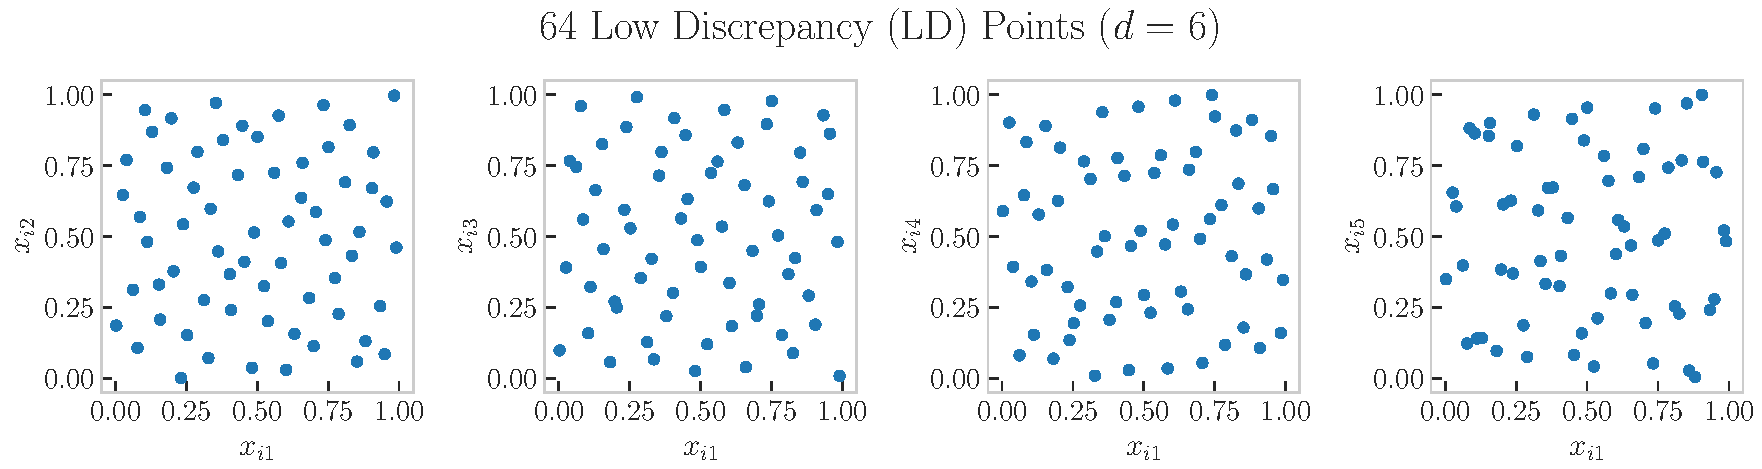
\includegraphics[width =\textwidth]{\figpath/64sobolpts_d6.pdf}
	\caption{LD points cover the unit cube even better than IID points or grids.  In any  projection there is  a similar looking distribution of all $64$ points. \label{fig:ld}}
\end{figure}


\section{LD Sequence Constructions} \label{sec:construct}
This section introduces some of the most popular LD sequences.  What sets these apart from IID sequences is that the nodes are deliberately chosen and highly correlated to one another, whether they be deterministic or randomized.

\subsection{Lattice Sequences} \label{sec:lattice}
One of the simplest LD constructions is the family of good lattice points \cite{DicEtal22a,SloJoe94}.  As a finite node set, they are defined as follows:
\begin{equation} \label{eq:latticepts}
	\bsx_i = i\bsh/n \pmod \bsone, \qquad i = 0, \ldots, n-1,
\end{equation}
where $\bsh$ is a well chosen $d$-dimensional integer vector. Figure \ref{fig:latticeconstruct} illustrates this construction for $n = 16$ and $\bsh = (1,11)$.  Note that the set $\{\bsx_0, \ldots, \bsx_{n-1}\}$ defined in \eqref{eq:latticepts} is closed under addition modulo $\bsone$ so that it forms a group.


\begin{figure}
	\centering
	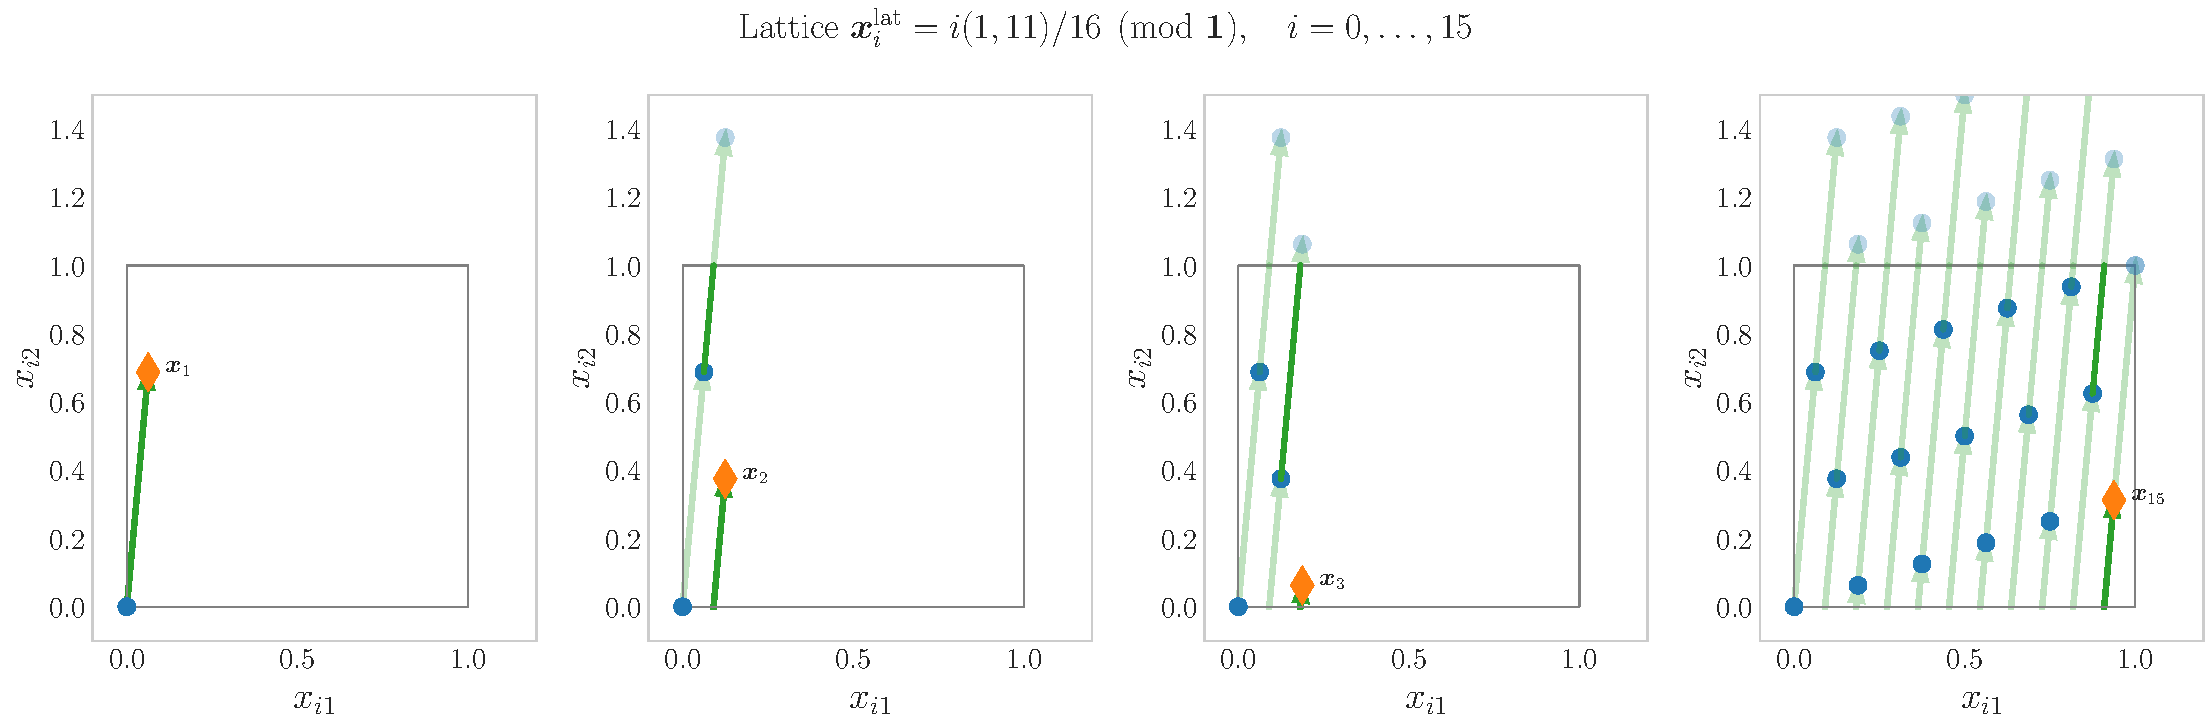
\includegraphics[width = \textwidth]{\figpath/16_lattice_construct_d2.pdf}
	\caption{The construction of a good lattice point set in two dimensions with $16$ nodes is obtained by moving $\bsh/n$ beyond the present point and wrapping around the boundaries of the square until one returns to the origin. \label{fig:latticeconstruct}}
\end{figure}


One disadvantage of this construction is that it is not readily extensible. For the example in Figure \ref{fig:latticeconstruct} the first $8$ points do not fill the unit square well.  However, the set of points defined by even $i$ do a reasonable job.  This suggests a method for defining extensible lattice sequences that was proposed independently by \cite{Mai81a} and \cite{HicEtal00}.

Let's start with the one-dimensional extensible lattice that is defined by the van der Corput sequence, $\{\phi_b(0), \phi_b(1), \ldots\}$.  This involves reflecting the digits of the integer $i$ in base $b$ about the decimal point.  For example, $\phi_2(6) = \phi_2(110_{2}) = {}_20.011 = 3/8$.  In general,
\begin{multline} \label{eq:vdc}
	\phi_b(i_0 + i_1b + i_2 b^2 + \cdots ) := i_0 b^{-1} + i_1 b^{-2} + i_2 b^{-3} + \cdots \in [0,1)
	\\
	 \text{where } i_0, i_1, \ldots \in \{0,\ldots b-1\}.
\end{multline}
For all non-negative integers, $m$, the first $n = b^m$ nodes in the van der Corput sequence correspond to the evenly spaced nodes $\{0, b^{-m}, \ldots, 1 - b^{-m} \}$---albeit in a different order.

To construct an extensible lattice, we replace $i/n$ in \eqref{eq:latticepts} by $\phi_b(i)$ to get
\begin{equation} \label{eq:extensiblelattice}
	\bsx_i =\phi_b( i)\bsh \pmod \bsone, \qquad i = 0, 1 , \ldots.
\end{equation}
This reordering of points from the original construction allows us to preserve the lattice structure for the first $b^m$ points for any non-negative integer $m$. That is, $\{\bsx_0, \ldots, \bsx_{2^m-1}\}$ is a closed under addition modulo $\bsone$.

Figure \ref{fig:extensiblelatticeconstruct} shows the first $4$, $8$, and $16$ points of the earlier example in Figure \ref{fig:latticeconstruct}.  The blue nodes are a copy of the nodes in the plot to the left, and the the orange nodes correspond to a shifted copy of the blue nodes modulo $\bsone$.  For the left plot, the shift is $\phi_2(2)\bsh = (1,11)/4$ or equivalently $(0.25,0.75)$.  For the middle plot, the shift is $\phi_2(4)\bsh = (1,11)/8$ or equivalently $(0.125,0.375)$. For the right plot, the shift is $\phi_2(8)\bsh = (1,11)/16$  or equivalently $(0.0625,0.6875)$.

\begin{figure}
	\centering
	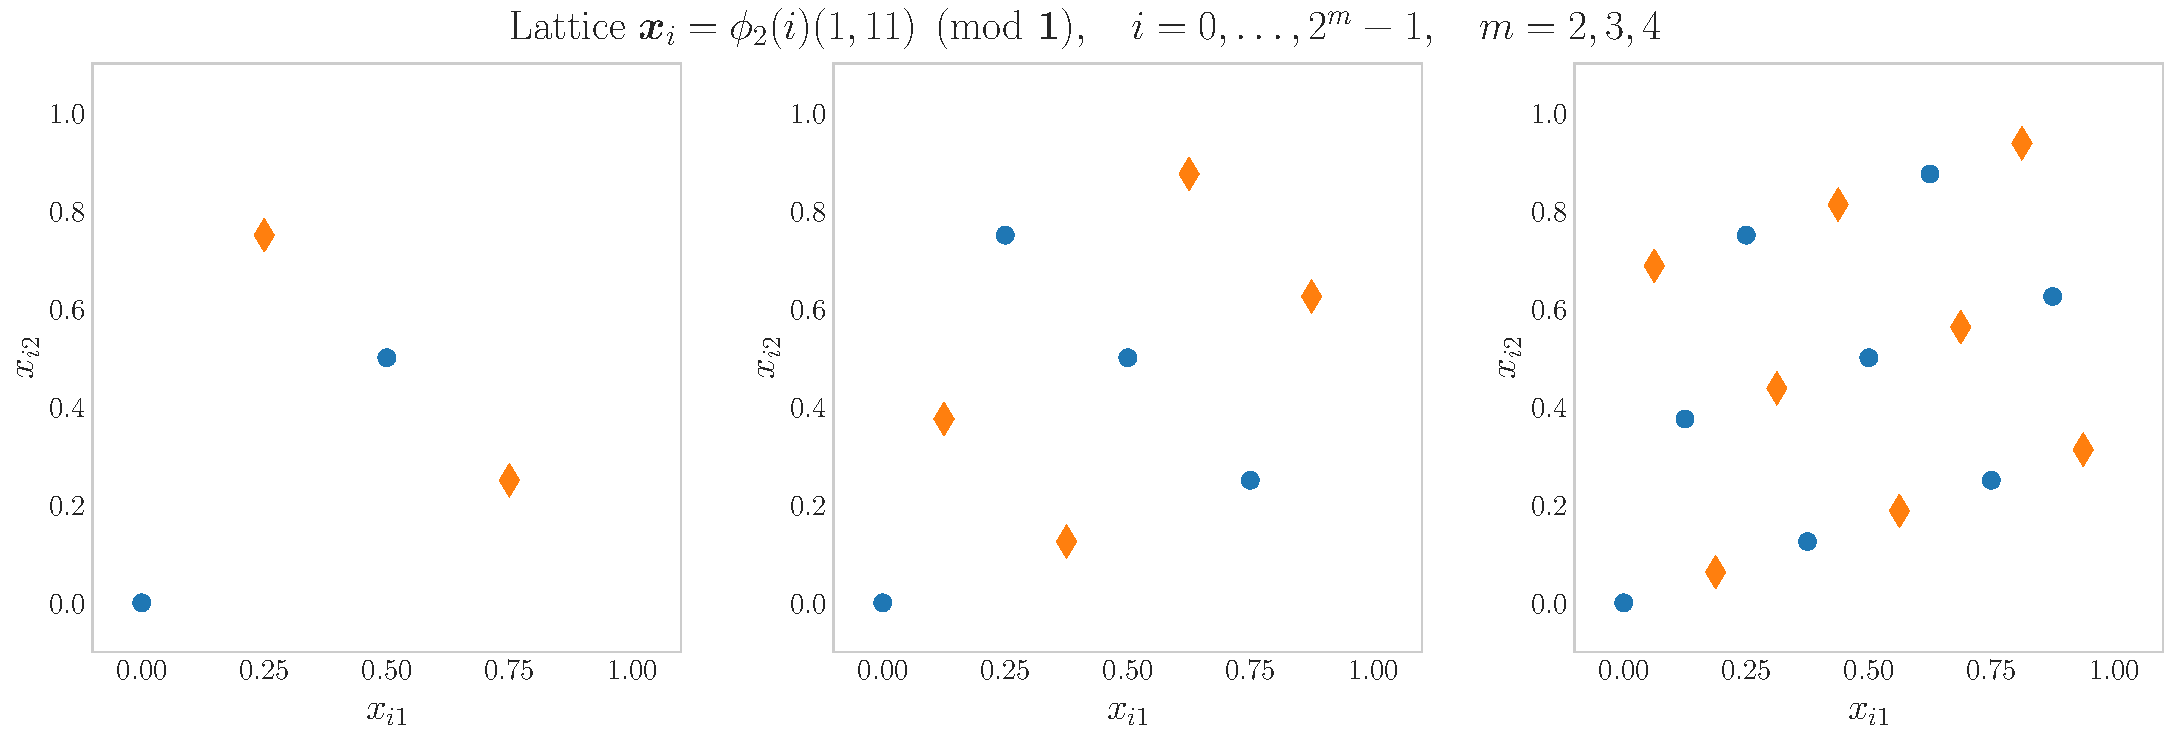
\includegraphics[width = \textwidth]{\figpath/16_extensible_lattice_construct_d2.pdf}
	\caption{An extensible lattice corresponding to  Figure \ref{fig:latticeconstruct}  with the nodes reordered using the van der Corput sequence in base $2$.  For each plot the blue nodes are a copy of the nodes to the left and the orange nodes are a shifted copy (modulo $\bsone$) of the blue nodes. \label{fig:extensiblelatticeconstruct}}
\end{figure}

For the example in Figure \ref{fig:extensiblelatticeconstruct}, increasing $n$ beyond $16$ repeats the original points because the generating vector $\bsh$ contains integers all less than $16$.  Obtaining a truly extensible lattice sequence requires that $\bsh$ be a vector of generalized integers---essentially integers with infinite numbers of nonzero digits---as explained in \cite{HicNie03a}, where the existence of good generating vectors is also proved.  In practice, one searches computationally for a $\bsh$ that produces good set of lattice nodes of size $n = b^m$ for a range of $m$ \cite{HicEtal00}.

The construction of great generating vectors for lattices has attracted a great deal of interest.  The component-by-component constructions pioneered by Frances Kuo, Josef Dick, Ian Sloan, Dirk Nuyens and others are surveyed in \cite[Chapter ?]{DicEtal22a}.  LatNet builder \cite{LEcEtal22a,LatNet} is a software package by Pierre L'Ecuyer and collaborators, which constructs generators for lattices and digital sequences.

\subsection{Digital Sequences} \label{sec:digital}

Another family of LD sequences also built upon the van der Corput sequence \eqref{eq:vdc} is digital sequences \cite{DicPil10a,Nie92}.  For simplicity, we restrict ourselves to $b = 2$ and let $\oplus$ denote binary digitwise addition modulo $2$ (also known as digitwise exclusive or), e.g., $3/8 \oplus 3/4 = {}_20.011 \oplus {}_20.110 = {}_20.101 = 5/8$.  A digital sequence is defined as
\begin{equation} \label{eq:digital}
	\bsx_i := i_0 \bsx_1 \oplus i_1 \bsx_2 \oplus i_2 \bsx_4 \oplus \cdots \in [0,1)^d \quad \text{for }
	i = i_0 + i_12 + i_2 2^2 + \cdots,
\end{equation}
where $\bsx_1, \bsx_2, \ldots$ are carefully chosen.  The node set $\{ \bsx_0, \ldots, \bsx_{2^m-1}\}$  for non-negative integer $m$ is called a digital net and is closed under $\oplus$.

If $x_{ij\ell}$ denotes the $\ell^{\text{th}}$ digit of the $j^{\text{th}}$ coordinate of $\bsx_i$, then the literature often defines generating matrices, $\mathsf{C}_j = (c_{ij\ell})_{\ell,i = 1}^{M,N}$ for $j = 1, \ldots, d$, where $M$ is the maximum number of bits in the expression for $\bsx_i$, say $52$, and $2^N$ is the maximum number of nodes that is intended to be generated.  The digital sequence can then be defined equivalently as
\begin{equation} \label{eq:digitalB}
	\begin{pmatrix} x_{ij1} \\ x_{ij2} \\ \vdots \end{pmatrix}
	= \mathsf{C}_j \begin{pmatrix} i_0 \\ i_1 \\ \vdots \end{pmatrix} \quad \pmod{2}, \qquad j = 1,\ldots, d, \ i = 0, 1, \ldots.
\end{equation}


To understand how these points might be evenly distributed over $[0,1)^d$, imagine a box of the form
\begin{multline} \label{eq:element_box}
	[a_1 b^{-k_1}, (a_1 + 1) 2^{-k_1}) \times \cdots \times [a_d b^{-k_d}, (a_d + 1) 2^{-k_d}), \\
	a_j \in \{0, \ldots, 2^{k_j} - 1\}, \ k_j \in \{0,1, \ldots \}, \qquad j =1, \ldots d.
\end{multline}
This box has volume $2^{-(k_1 + \cdots +k_d)} = 2^{-\lVert\bsk\rVert_1}$.  For a digital net with $2^m$ points and $m \ge \lVert \bsk \rVert_1$, a ``fair share" of nodes for this box would be $2^{m- \lVert \bsk \rVert_1}$.  This will occur if and only if
\begin{multline} \label{eq:tcond}
	\text{the first $k_1$ rows of the first $m$ columns of $\mathsf{C}_1$ plus} \\
	\text{the first $k_2$ rows of the first $m$ columns of $\mathsf{C}_2$ plus} \\
	 \cdots \\
	\text{the first $k_d$ rows of the first $m$ columns of $\mathsf{C}_d$} \\
	\text{are linearly independent over the finite field with the elements $\{0,1\}$, }
\end{multline}
regardless of the choice of $\bsa = (a_1, \ldots, a_d)$.  The $t$-value of a digital net with $2^m$ nodes is defined as the smallest $t$ for which condition \eqref{eq:tcond} holds for all $\bsk$ with $\lVert \bsk \rVert_1 \le m-t$.  Equivalently, this $t$ is the smallest value for which every box of the form \eqref{eq:element_box} with volume $2^{\lVert \bsk \rVert_1 - m}$ contains its fair share of $2^t$ nodes.  Such a digital net is then called a $(t,m,d)$-net.  An infinite sequence of the form \eqref{eq:digitalB} for which this condition holds for all non-negative $m$ is called a  $(t,d)$-sequence.

To illustrate the $t$-value, consider the following digital net with $2^3$ (eight) nodes, i.e., $m = 3$:
\begin{multline} \label{eq:smallnet}
	\{(0, 0,   0),
	(0.5,   0.5,   0.5  ),
	(0.25,  0.75,  0.75 ),
	(0.75,  0.25,  0.25 ),
	(0.125, 0.625, 0.375),\\
	(0.625, 0.125, 0.875),
	(0.375, 0.375, 0.625),
	(0.875, 0.875, 0.125)\}.
\end{multline}
Figure \ref{fig:elementinterval} shows several two dimensional projections of these nodes and the two-dimensional boxes (rectangles) of the form \eqref{eq:element_box} with $\lVert\bsk\rVert_1 = 3$.  Most of the boxes contain their fair share of one node, but the box $[0,1/4) \times [0,1) \times [0,1/2)$ contains two nodes and the adjacent box, $[1/4,1/2) \times [0,1) \times [0,1/2)$ contains no nodes.  Thus, the $t$-value cannot be $0$.  However, the $t$-value is $1$ because all boxes of the form  \eqref{eq:element_box} with $\lVert\bsk\rVert_1 = 2$, i.e., a volume of $2^{-2} = 1/4$ contain a fair share of $2^{m- \lVert \bsk \rVert_1} = 2$ points.  The node set \eqref{eq:smallnet} is a $(1,3,3)$-net.

This conclusion can also be reached by looking at the first three rows and columns of the generating matrices for this digital net, which are
\begin{equation*}
	\mathsf{C}_1 = \begin{pmatrix}
		1 & 0 & 0 & \cdots \\ 0 & 1 & 0 & \cdots \\ 0 & 0 & 1 & \cdots \\ \vdots & \vdots & \vdots & \ddots
	\end{pmatrix}, \quad
	\mathsf{C}_2 = \begin{pmatrix}
		1 & 1 & 1 & \cdots \\ 0 & 1 & 0 & \cdots \\ 0 & 0 & 1 & \cdots \\ \vdots & \vdots & \vdots & \ddots
	\end{pmatrix}, \quad
	\mathsf{C}_3 = \begin{pmatrix}
	1 & 1 & 0 & \cdots \\ 0 & 1 & 1 & \cdots \\ 0 & 0 & 1 & \cdots \\ \vdots & \vdots & \vdots & \ddots
\end{pmatrix}.
\end{equation*}
For $k_1=2$, $k_2 = 0$, and $k_3 = 1$ condition \eqref{eq:tcond} is not satisfied, and so $t$ cannot be $0$ for the node set  \eqref{eq:smallnet}.  However, condition \eqref{eq:tcond} is satisfied for all $\bsk$ with $\lVert \bsk \rVert_1 = 2$, again confirming that we have a $(1,3,3)$-net.

If we consider only the first two coordinates of the node set defined in \eqref{eq:smallnet}, then  condition \eqref{eq:tcond} is satisfied for all $\bsk$ with $\lVert \bsk \rVert_1 = 3$.  The first two coordinates of \eqref{eq:smallnet} are a $(0,3,2)$-net



\begin{figure}
	\centering
	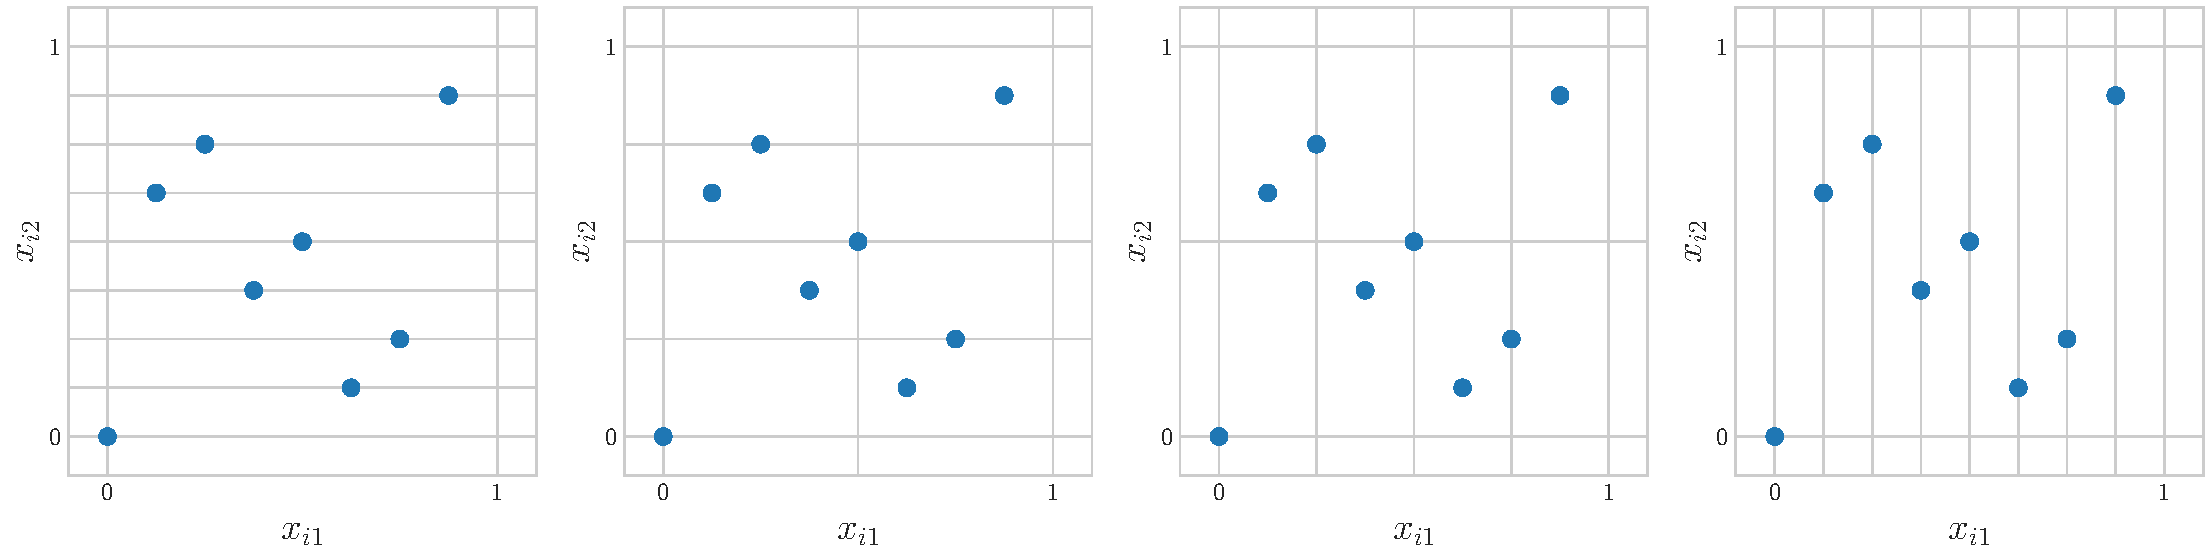
\includegraphics[width = \textwidth]{\figpath/8_sobol_sequence_elementary_intervals_d3_coord_(1,2)}
	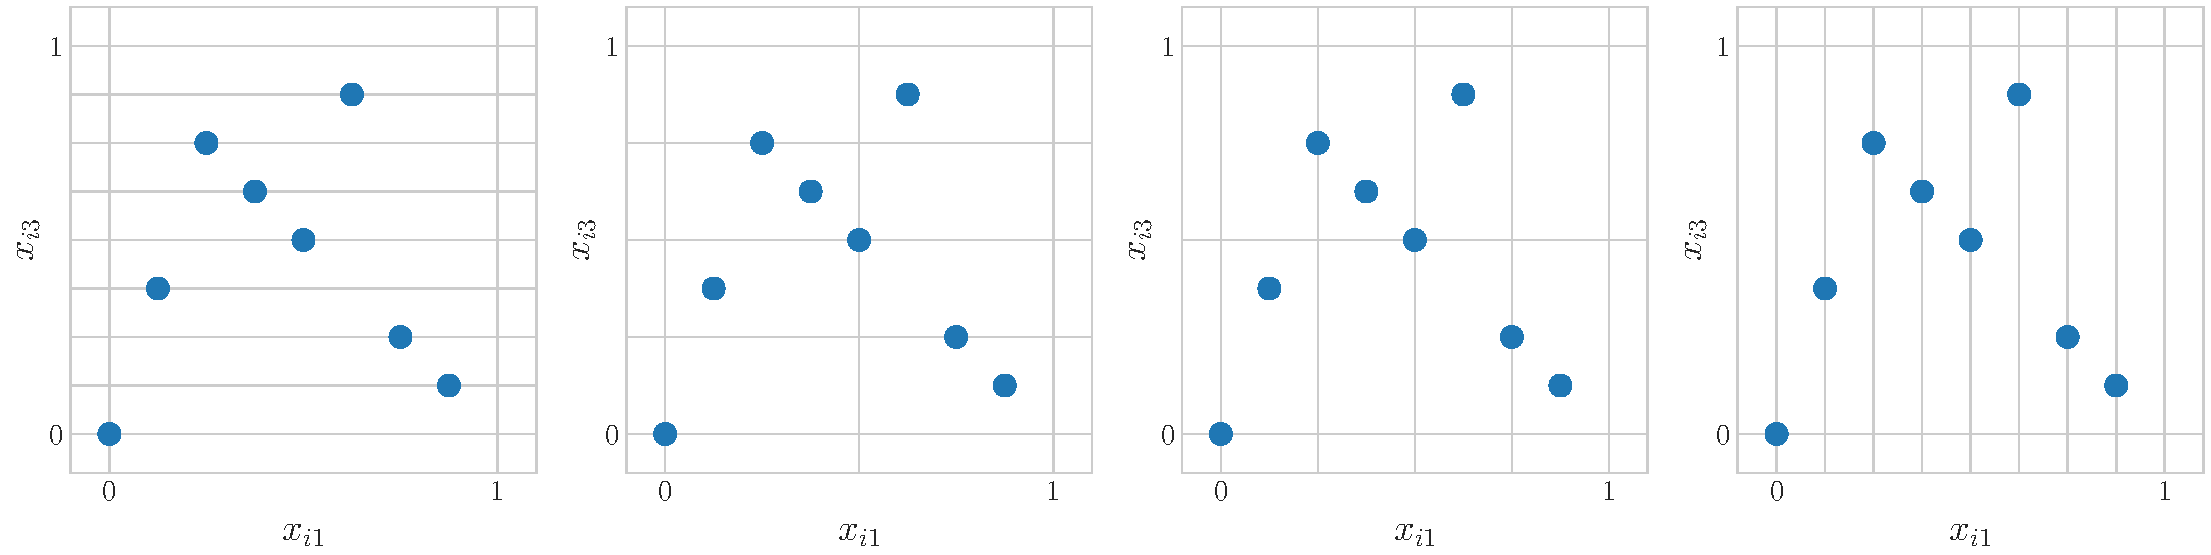
\includegraphics[width = \textwidth]{\figpath/8_sobol_sequence_elementary_intervals_d3_coord_(1,3)}
	\caption{Each box in the two dimensional projections of the node set \eqref{eq:smallnet} plotted above show one point in each box except for the second row, third plot from the left.  Thus, this node set is not a $(0,3,3)$-net.  It is however a $(1,3,3)$-net.  \label{fig:elementinterval}}
\end{figure}



Digital sequence generators can be found via number theory or numerical search \cite{}.  The earliest instance is due to Sobol' \cite{}.

\subsection{Halton sequences} \label{sec:Halton}  While lattice sequences and digital sequences have preferred sample sizes, $n$, Halton sequences have no preferred sample size.  The Halton sequence is defined in terms of the van der Corput sequence
\begin{equation}\label{eq:Halton}
	\bsx_i = \bigl( \phi_{b_1}(i), \ldots, \phi_{b_d}(i) \bigr), \qquad i = 0, 1, \ldots,
\end{equation}
where $b_1, \ldots, b_d$ is a choice of $d$ distinct prime numbers.  Often they are chosen as the first $d$ prime numbers.  Figure \ref{fig:Halton} shows two dimensional projections of Halton points

\begin{figure}
	\centering
	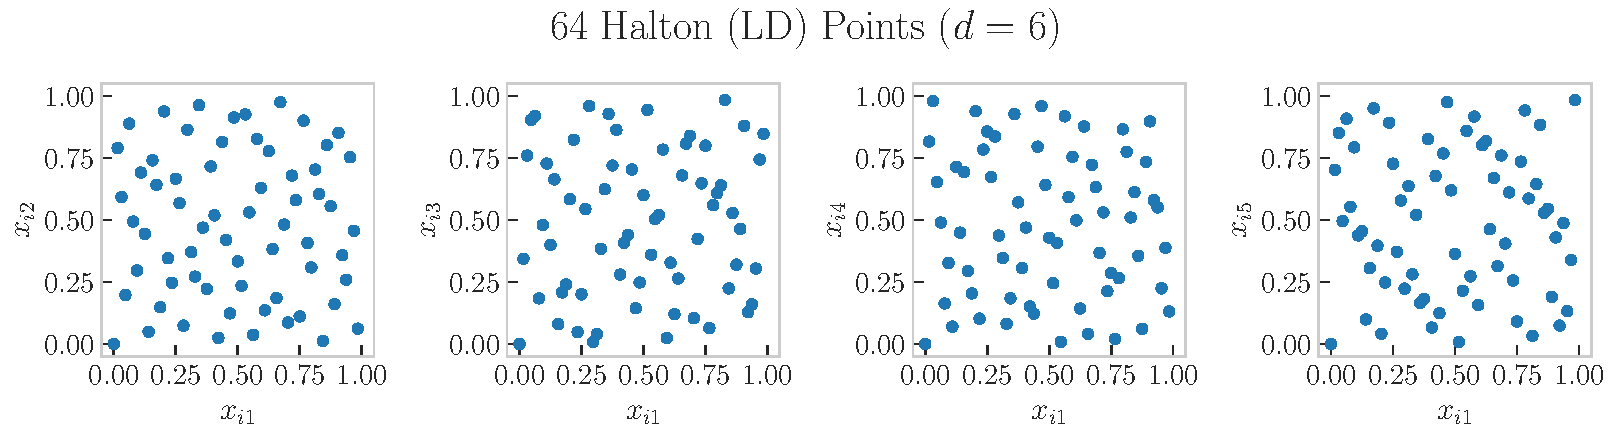
\includegraphics[width=\textwidth]{\figpath/64Halton_pts_d6.pdf}
	\caption{Halton points as defined in \eqref{eq:Halton} have low discrepancy but no preferred sample size. \label{fig:Halton}}
\end{figure}

\subsection{LD Nodes by Optimization}\label{sec:optLD}

Most quasi-Monte Carlo constructions are studied based on their asymptotic behavior as \(n \to \infty\), with numerous results on asymptotic rates \cite{NIED1978QMCBook,NovWoz10a}. However, few methods address finding optimal point configurations for specific \(n\) and \(d\) which can be critical in practical applications where each function evaluation is costly. Of course, one possible strategy is to truncate asymptotically optimal sequences to the desired \(n\), however, as discussed above many of the standard LD constructions have a preferred number of points with truncations leading to imbalances in equidistribution. We can often do better optimizing directly for the target \(n\) and \(d\).

%When optimizing a sample point distribution, one requires a figure-of-merit to serve as the objective function for the optimization problem.

\vspace{2mm}
\noindent
\textbf{Combinatorial Optimization.}
For several decades, combinatorial optimization techniques have been employed to obtain good generating vectors for rank-1 lattice points. Recall that for given \(n\) and \(d\), a lattice rule is fully determined by the generating vector \(\boldsymbol{h} \in \mathbb{Z}_n^d \coloneqq \{0, 1, \ldots, n-1\}^d\). While good generating vectors are known for \(d \leq 2\) \cite{DicEtal22a,SloJoe94}, the same does not hold for \(d \geq 3\), often resorting to finding good $\boldsymbol{h}$ via computer search to minimize a chosen figure-of-merit. An exhaustive search is infeasible due to the exponential growth of the search space with \(d\). The component-by-component (CBC) construction, introduced by Korobov \cite{kor63} and later revisited by Sloan and collaborators \cite{Slo02}, reduces the search space to size \(dn\) by constructing \(\boldsymbol{h}\) one component at a time.
%Further simplification is possible by restricting the search to Korobov lattices of the form \(\boldsymbol{h} = (1, h, h^2, \ldots, h^{d-1}) \in \mathbb{Z}^d\).
For certain choices of function spaces, there exist fast component-by-component construction implementations using fast Fourier transforms (FFTs) as the primary tool. We refer to \cite{DicKuo04a,JoeKuo03,KuoJoe02b} and references therein for works on the CBC construction for lattice rules and \cite{NuyCoo06a,NuyCoo06b} for their fast implementations.



\vspace{2mm}
\noindent
\textbf{Global Optimization.}



\vspace{2mm}
\noindent
\textbf{Other Notable Methods.}




\section{Randomization} \label{sec:random}
The LD constructions described in the previous section have so far been \emph{deterministic}. The sample mean, $\hat{\mu}_n$, does not change each time it is computed like it would for IID nodes.

While determinism has some advantages, randomization has advantages as well.
\begin{itemize}
	\item Randomization done right removes bias in the estimator.
	\item Replications of random estimators can facilitate error estimates for the sample mean.
	\item Often the application of interest requires transforming the LD nodes to mimic other distributions.  This is the case in the Keister example of Section \ref{sec:intro}, as seen in \eqref{eq:sample_mean_Keister}.  There the nodes, $\{\bsx_i\}_{i=0}^{n-1}$, are transformed to mimic a Gaussian distribution.

	The LD sequences defined in the previous section start with $\bsx_0 = \bszero$, as can be seen in \eqref{eq:latticepts}, \eqref{eq:digital}, \eqref{eq:Halton}, and Figures \ref{fig:latticeconstruct}--\ref{fig:Halton}.  The node $\bszero$ becomes infinite under a transformation to mimic a Gaussian distribution, which can trigger runtime errors.  Randomization eliminates nodes on the boundary of the unit cube.
\end{itemize}
The key to good randomization is to preserve the LD quality of the node sequence.

\subsection{Shifts} \label{sec:shifts}
The simplest randomization is to shift the node sequence by $\bsDelta  \sim \calU[0,1)^d$.  For lattice  sequences the shift is applied modulo $\bsone$ so that shifted extensible lattice turns
\eqref{eq:extensiblelattice} into
\begin{equation} \label{eq:sh_extensiblelattice}
	\bsx^{\bsDelta\text{-lat}}_i := \bsx_i + \bsDelta \pmod \bsone =\phi_b( i)\bsh + \bsDelta \pmod \bsone, \qquad i = 0, 1 , \ldots.
\end{equation}
Since the first $2^m$ elements of the lattice sequence form a group under modulo $\bsone$ addition, the coresponding shifted node set is a coset.  Figure \ref{fig:shift_lat} illustrates three shifts of the lattice plotted in Figure \ref{fig:latticeconstruct}.

\begin{figure}
	\centering
	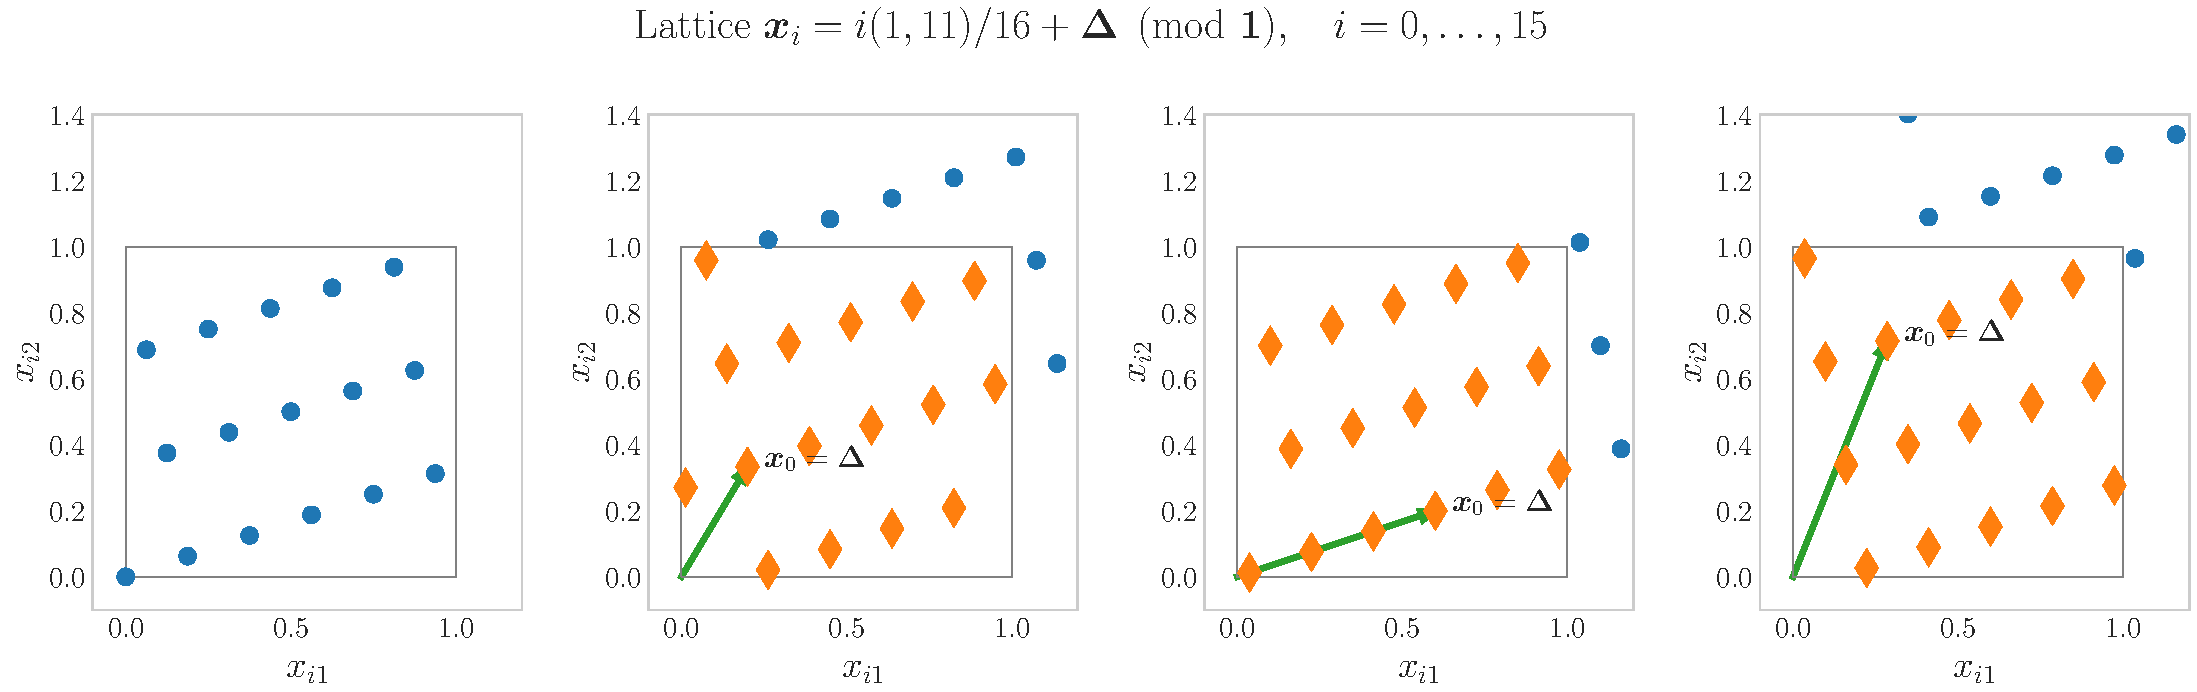
\includegraphics[width = \textwidth]{\figpath/16_shifted_lattice_construct_d2.pdf}
	\caption{The original unshifted lattice (left) and three different shifts modulo $\bsone$ of the lattice.  Note that the structure of the lattice is maintained. \label{fig:shift_lat}}
\end{figure}

For digital sequences the shift should be applied using digitwise addition.  A digital shift of the digital sequence defined in  \eqref{eq:digital} then becomes
\begin{equation} \label{eq:sh_digital}
	\bsx_i^{\bsDelta\text{-dig}} := \bsx_i \oplus \bsDelta = i_0 \bsx_1 \oplus i_1 \bsx_2 \oplus i_2 \bsx_4 \oplus \cdots \oplus \bsDelta \in [0,1)^d \quad \text{for }
	i = i_0 + i_12 + i_2 2^2 + \cdots.
\end{equation}
Three digital shifts of the same net are given in Figure \ref{fig:shift_net}.  A digital shift does not alter the $t$-value of a $(t,m,d)$-net.

\begin{figure}
	\centering
	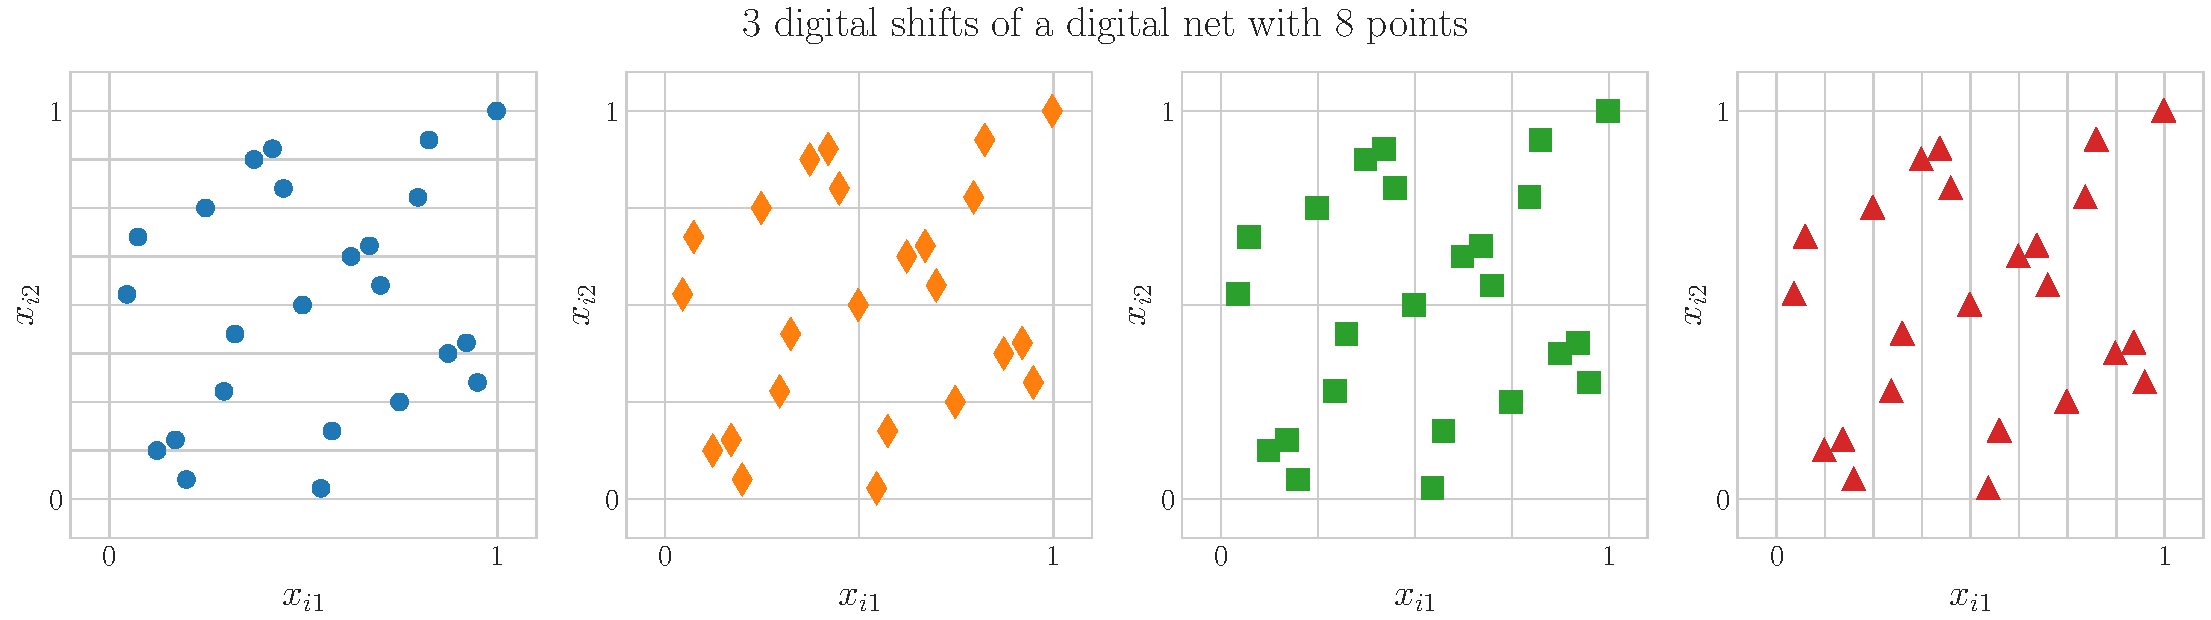
\includegraphics[width = \textwidth]{\figpath/n_8_n_sh_3_shifted_sobol_sequence_d2.pdf}
	\caption{Three digital shifts of a digital $(0,3,2)$-net with nodes denoted by three different colors.  There is one node in each smaller box of the form \eqref{eq:element_box} for $\lVert \bsk \rVert = 3$, for each digitally shifted net. \label{fig:shift_net}}
\end{figure}

Let $\{\bsx_i^{\bsDelta}\}_{i=0}^{n-1}$ denote a random shift of any deterministic original node set, $\{\bsx_i \}_{i=0}^{n-1}$ as described above.  That is, $\bsx_i^{\bsDelta} : = \bsx_i + \bsDelta \pmod \bsone$ or  $\bsx_i^{\bsDelta} : = \bsx_i \oplus \bsDelta$ and $\bsDelta \sim \calU[0,1)^d$. This then implies that each $\bsx_i^{\bsDelta} \sim \calU[0,1)^d$ and thus $\hat{\mu}_n$ is an unbiased estimator of $\mu$, which was mentioned at the beginning of this section.

\subsection{Digital Scrambles} \label{sec:scrambles}
For digital nets one can randomize even further by a scrambling that preserves the $t$-value.  Owen \cite{Owe95} proposed a scrambling of nets called nested uniform scrambling.  A simpler version called linear matrix scrambling was proposed by Matou\v{s}ek \cite{Mat98} and is described here.  Starting from the formulation of digital sequences involving generator matrices in \ref{eq:digitalB}, we multiply each generator matrix on the left by a lower triangular matrix with ones along the diagonals and elements below the diagonal that are randomly chosen to be $0$ or $1$ with equal probability:
\begin{subequations} \label{eq:scr_lattice}
\begin{gather} \label{eq:digitalscr}
	\begin{pmatrix} x^{\text{scr}}_{ij1} \\ x^{\text{scr}}_{ij2} \\ \vdots \end{pmatrix}
	= \mathsf{L_j} \mathsf{C}_j \begin{pmatrix} i_0 \\ i_1 \\ \vdots \end{pmatrix} + \begin{pmatrix} \Delta_{1j} \\ \Delta_{2j} \\ \vdots \end{pmatrix} \quad \pmod{2}, \qquad j = 1,\ldots, d, \ i = 0, 1, \ldots, \\
	\mathsf{L_j} :=
	\begin{pmatrix}
		1 & 0 & 0 & 0 & \cdots \\
		l_{21} & 1 & 0 & 0 & \cdots \\
		l_{31} & l_{32} & 1 & 0 & \cdots \\
		\vdots & \vdots & \vdots & \ddots & \ddots
	\end{pmatrix}, \qquad l_{\ell j} \overset {\text{IID}}{\sim} \calU\{0,1\}
\end{gather}
\end{subequations}
A random digital shift, $\bsDelta$ is also added, where $\Delta_{\ell j}$ denotes the $\ell^{\text{th}}$ digit of the $j^{\text{th}}$ of the shift.

\begin{figure}
	\centering
	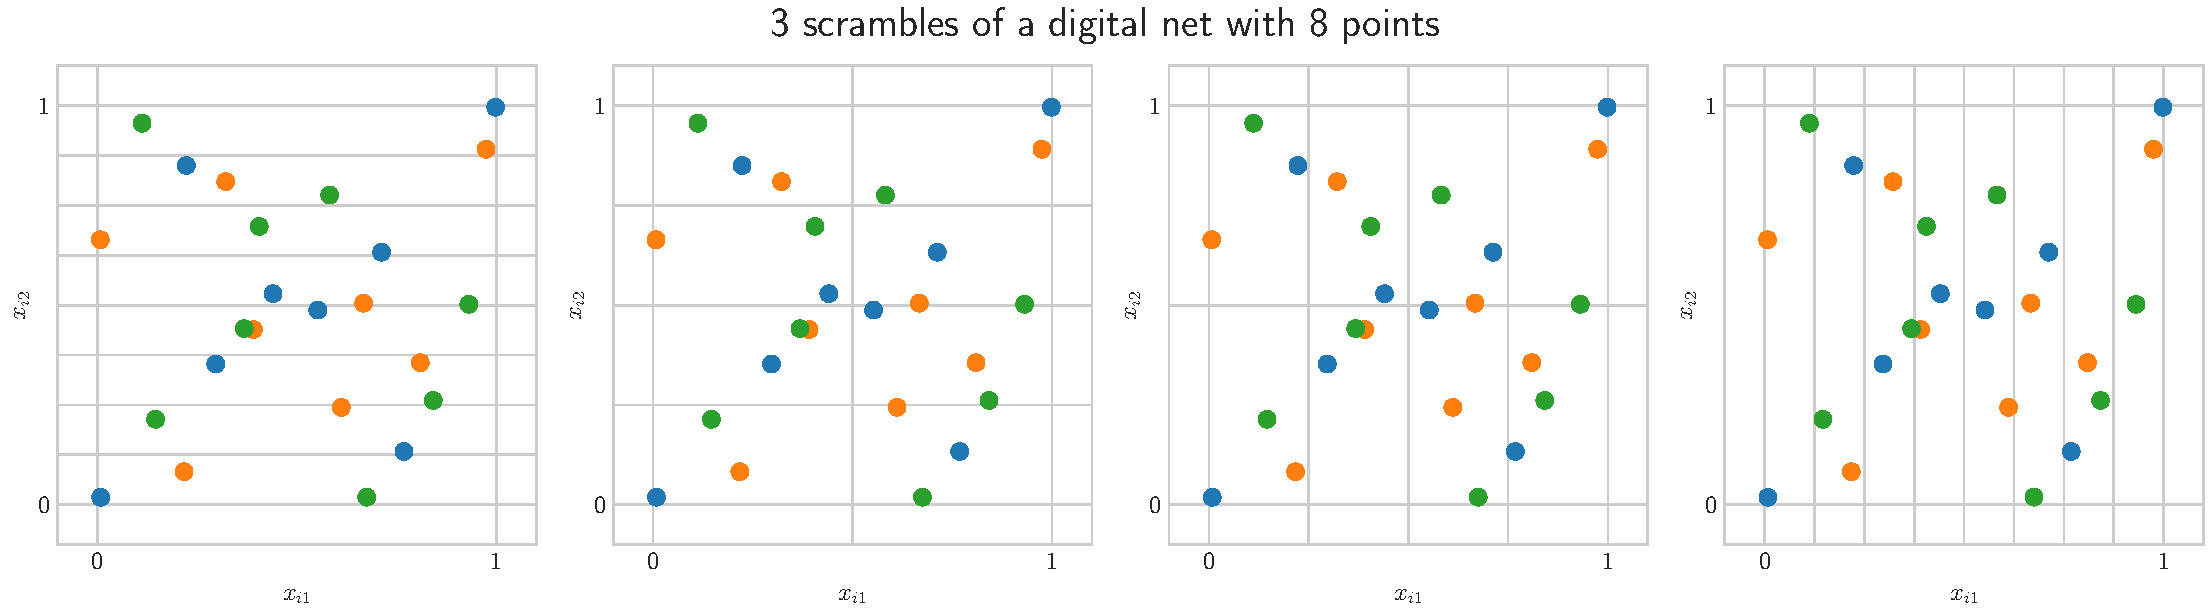
\includegraphics[width = \textwidth]{\figpath/n_8_n_scr_3_scrambled_sobol_sequence_d2.pdf}
	\caption{Three linear scrambles of a digital $(0,3,2)$-net with nodes denoted by three different colors.  There is one node in each smaller box of the form \eqref{eq:element_box} for $\lVert \bsk \rVert = 3$, for each digitally shifted net. \label{fig:scrambled_net}}
\end{figure}

[make a scramble of an image]

\subsection{Other Randomizations for Halton}

\subsection{Randomized Generators}


\section{Discrepancy} \label{sec:discrepancy}
So far, we have relied on eye tests and the Keister example to show how LD sequences are better than IID.  This section introduces the theory that shows way minimizing discrepancy leads to better approximations to $\mu$.


\subsection{Discrepancies Defined by Kernels} \label{sec:kerdisc}
Let $K: [0,1)^d \times [0,1)^d \to \mathbb{R}$ be a function satisfying the following two conditions:
\begin{subequations} \label{eq:Kcond}
	\begin{align}
		\label{eq:KcondSym}
		\text{Symmetry:} \quad & K(\bst,\bsx) = K(\bsx,\bst) \qquad \forall \bst,\bsx \in [0,1)^d \\
		\nonumber
		\text{Postitive definiteness:} \quad & \sum_{i,j = 0}^{n-1} c_i K(\bsx_i,\bsx_j) c_j > 0 \qquad  \forall n \in \mathbb{N}, \ \bsc \ne 0, \\
		& \qquad \qquad  \ \text{distinct } \bsx_0, \ldots, \bsx_{n-1} \in [0,1)^d. \label{eq:KcondPD}
	\end{align}
\end{subequations}
Then it is known \cite{Aro50} that this $K$ is the reproducing kernel for a Hilbert space, $\calH_K$ with associated inner product $\langle \cdot, \cdot \rangle_{\calH_K}$, such that
\begin{subequations}
	\begin{align}
	\text{Belonging:} \quad & K(\cdot,\bsx) \in \calH_K \qquad \forall \bsx \in [0,1)^d \\
	\text{Reproducing:} \quad & f(\bsx) = \langle K(\cdot,\bsx),f \rangle \qquad  \forall \bsx \in [0,1)^d, \ f \in \calH_K.
\end{align}
\end{subequations}

Having a reproducing kernel Hilbert space with a known kernel $K$ allows us to derive a rigorous error bound for $\mu - \hat{\mu}_n$.  First note that for any bounded, linear functional, $L$ on the Hilbert space $\calH_K$, there is some $\eta_L \in \calH_K$ such that
\begin{equation*}
L(f) = \langle \eta_L , f \rangle_{\calH_K} \qquad \forall f \in \calH_K.
\end{equation*}
This is guaranteed by the Riesz Representation Theorm, and $\eta_L$ is called the representer of $L$.  Using the reproducing property of $K$, one may derove am explict formula for $\eta_L(\bsx)$, namely,
\begin{equation*}
\eta_L(\bsx) = \langle K(\cdot, \bsx), \eta_L \rangle_{\calH_K} = L\bigl( K(\cdot,\bsx) \bigr).
\end{equation*}
From this expression for $\eta_L(\bsx)$ one may then calculate the squared norm of the linear functional $L$ as the squared norm of its representer:
\begin{equation} \label{eq:sqnormL}
	\lVert \eta_L \rVert_{\calH_K}^2 = \langle\eta_L, \eta_L \rangle_{\calH_K} = L(\eta_L) = L^{\cdot\cdot} \Bigl(L^{\cdot}\bigl( K(\cdot,\cdot \cdot) \bigr) \Bigr).
\end{equation}

If $\mu(\cdot)$ is a bounded linear functional on $\calH_K$ is, we may use the argument above to derive our error bound.  First we write the dependence of $\mu - \hat{\mu}_n$ on  $f$ explicitly as $\mu(f) - \hat{\mu}_n(f)$ and note that the error functional, $\mu(\cdot) - \hat{\mu}_n(\cdot)$, is  linear.  The Riesz Representation Theorem and the Cauchy-Schawarz inequality imply a tight error bound:
\begin{align}
	\nonumber
	\lvert\mu(f) - \hat{\mu}_n(f) \rvert
	& = \lvert \langle \eta_{\mu(\cdot) - \hat{\mu}_n(\cdot)}, f \rangle_{\calH_K} \rvert
	 \le \lVert  \eta_{\mu(\cdot) - \hat{\mu}_n(\cdot)} \rVert_{\calH_K} \, \lVert f \rVert_{\calH_K}\\
	\lvert\mu(f) - \hat{\mu}_n(f) \rvert
	& \le \underbrace{\lVert  \eta_{\mu(\cdot) - \hat{\mu}_n(\cdot)} \rVert_{\calH_K}}_{=:\text{discrepancy}\bigl(\{\bsx\}_{i=0}^{n-1},K \bigr)}
	\, \underbrace{\inf_{c \in \RR}\lVert  f - c \rVert_{\calH_K}}_{=:\text{variation}(f,K)} \qquad \forall f \in \calH_K,  \label{eq:cuberrbd}
	\intertext{since $\hat{\mu}_n$ is exact for constants.  (It is assumed that $\calH$ contains constant functions so that $f \in \calH_K$ implies that $f - c \in \calH_K$.)  The squared norm of the error funtional can be expressed explicitly via \eqref{eq:sqnormL} as}
	\nonumber
	\text{discrepancy}^2\bigl(\{\bsx\}_{i=0}^{n-1},K \bigr) & = \lVert  \eta_{\mu(\cdot) - \hat{\mu}_n(\cdot)} \rVert_{\calH_K}^2 \\
	\nonumber
	& =
	\bigl(\mu(\cdot\cdot) - \hat{\mu}_n(\cdot\cdot)\bigr) \Bigl(\bigl(\mu(\cdot) - \hat{\mu}_n(\cdot)\bigr)\bigl( K(\cdot,\cdot \cdot) \bigr) \Bigr) \\
	\nonumber
	& = \int_{[0,1)^d \times [0,1)^d} K(\bst,\bsx) \, \mathrm{d} \bst \, \mathrm{d} \bsx  -\frac 2n  \sum_{i=0}^{n-1} \int_{[0,1)^d} K(\bst,\bsx_i) \, \mathrm{d} \bst \\
	& \qquad \qquad + \frac{1}{n^2} \sum_{i,j=0}^{n-1}  K(\bsx_i,\bsx_j). \label{eq:sqdisc}
\end{align}

Error bound \eqref{eq:cuberrbd} has two factors:
\begin{itemize}
	\item the discrepancy, which is the norm of the error functional, is a measure of deficiency of the node set, $\{\bsx\}_{i=0}^{n-1}$, and
	\item the variation is a measure of the roughness of the function defining our random variable whose expectation we wish to compute.
\end{itemize}
In general, designers of qMC methods want to construct sets or sequences of nodes with  discrepancy as small as possible, either by increasing $n$, if the computational budget allows, or by better placement of the nodes.  The constructions described in Section \ref{sec:construct} are ways of ensuring better placement of the nodes, provided that the generators are chosen well.  Practitioners of qMC want to formulate $\mu$ in a way to make the variation as small as possible.  This discussed in Section \ref{sec:reformulate}.

Although error bound \eqref{eq:cuberrbd} is elegant, it leaves several matters unresolved:
\begin{itemize}
	\item The reproducing kernel $K$ defines both the discrepancy and the variation.  This means that differnt choices of $K$ will lead to different error bounds for the same $\hat{\mu}_n$, even though the error is unchanged.
	\item The Hilbert space $\calH_K$ contains ones assumptions about $f$, such as smoothness or periodicity. Knowing $K$, however, does not automatically lead to an explict formula for the inner product of the associated Hilbert space, $\langle \cdot, \cdot \rangle_{\calH_K}$.  Conversely, having an explict formula for  $\langle \cdot, \cdot \rangle_{\calH_K}$ does not automatically lead to an explict formula for the reproducing kernel, $K$.  In both cases educated guesswork is involved.
	\item Choosing a more restrictive $\calH_K$ may lead to a sharper error bound, however, it is often infeasible in practice to check whether the ``black box'' $f$ lies in $\calH_K$.
	\item   Moreover, even if one is confident that $f \in \calH_K$, it is usually impractical to compute variation$(f,K)$, as we shall see below.  Error bound \eqref{eq:cuberrbd} cannot be used as a stopping criterion to determine the $n$ needed to satisfy an error tolerance.
\end{itemize}
In spite of these drawbacks, \eqref{eq:cuberrbd} is quite useful:
\begin{itemize}
	\item There are a family of commonly used reproducing kernels \cite{BerT-A04,Hic97a,Hic98b,Hic99b}. Once $K$ has been fixed, the discrepancy may be used as a comparison measure among different LD sequences, and its rate of decay---which sometimes can be computed theoretically---indicates how quickly $\hat{\mu}_n$ approaches $\mu$.
	\item When an explict formula for the inner product of the associated Hilbert space, $\langle \cdot, \cdot \rangle_{\calH_K}$ can be deduced, it suggests how to $\mu$ to reduce variation$(f)$.
\end{itemize}

\subsection{The Centered Discrepancy}
An example of a reproducing kernel defined on $[0,1)^d \times [0,1)^d$ is
\begin{equation} \label{eq:ctrkernel}
	K(\bst,\bsx) = \prod_{\ell = 1}^d \left[ 1 + \frac 12 \bigl ( \lvert t_\ell - 1/2 \rvert + \lvert x_\ell - 1/2 \rvert - \lvert t_\ell - x_\ell \rvert \bigr ) \right] .
\end{equation}
One can easily see that this $K$ satisfies the symmetry condition \eqref{eq:KcondSym}.  It also is symmetric about the middle of the unit cube, i.e.,
\begin{equation*}
	K\bigl((t_1,\ldots, t_{\ell-1}, 1 - t_\ell,  t_{\ell+1}, \ldots, t_d),
	(x_1,\ldots, x_{\ell-1}, 1 - x_\ell,  x_{\ell+1}, \ldots, x_d)
	\bigr) =
	K(\bst,\bsx),
\end{equation*}
which is a desirable property for problems where there is no preferred corner.

The inner product for the Hilbert space $\calH_K$ with reproducing kernel $K$ is
\begin{align}
	\langle f, g \rangle_{\calH_K} &= f(\boldsymbol{1/2}) g(\boldsymbol{1/2}) \nonumber
	\\
	&
	+ \int_{[0,1)} [D^{\{1\}}f](x_1) \, [D^{\{1\}}g](x_1)\, \mathrm{d} x_1
	+ \int_{[0,1)} [D^{\{2\}}f](x_2) \, [D^{\{2\}}g](x_2)\, \mathrm{d} x_2 \nonumber \\
	& \qquad \qquad + \cdots \nonumber\\
	&
	+ \int_{[0,1)^2} [D^{{\{1,2\}}}f](x_1,x_2) \, [D^{\{1,2\}}g](x_1,x_2)\, \mathrm{d} x_1 \mathrm{d} x_2 + \cdots \nonumber \\
	&  \qquad \qquad + \cdots + \int_{[0,1)^d} [D^{\{1,\ldots, d\}}f](\bsx) \, [D^{\{1,\ldots, d\}}g](\bsx) \, \mathrm{d} \bsx \nonumber \\
	& = \sum_{\bsell \subseteq \{1, \ldots, d\}} \langle D^{\bsell}f, D^{\bsell}g \rangle_2
\end{align}
where $\langle \cdot,\cdot \rangle_2$ denotes the $L^2$ inner product,
\begin{multline*}
	[D^{\{\ell_1, \ell_2, \ldots, \ell_s\} }f](x_1, x_2, \ldots, x_s) \\
	: = \frac{\partial^s f(1/2,\ldots, 1/2, x_{\ell_1}, 1/2, \ldots, 1/2, x_{\ell_2}, 1/2, \ldots, 1/2, x_{\ell_s}, 1/2, \ldots, 1/2)}{\partial x_{\ell_1} \partial x_{\ell_2} \cdots \partial x_s},
\end{multline*}
and $D^{\emptyset}f$ is understood to be the constant $f(1/2, \ldots, 1/2)$ \cite{Hic97a}.  The variation, which corresponds to the non-constant part of the function, is
\begin{equation*}
		\text{variation}(f) := \sqrt{\sum_{\emptyset \ne \bsell \subseteq \{1, \ldots, d\}} \lVert D^{\bsell}f\rVert_2^2}.
\end{equation*}

We show that $K$ defined in \eqref{eq:ctrkernel} is the reproducing kernel for the $\calH_K$ with the above inner product for $d=1$ and assuming $0 \le x \le 1/2$:
\begin{align*}
	\langle K(\cdot,x), f \rangle_{\calH_K}
	& =
	K(1/2,x) f(1/2) + \int_0^1 \frac{\partial K(t,x)}{\partial t} f'(t) \, \mathrm{d} t \\
	& = 1 \times f(1/2) +  \int_0^x \frac 12 [-1  - (-1) ] f'(t) \, \mathrm{d} t +
	\int_x^{1/2} \frac 12 [-1  - 1 ] f'(t) \, \mathrm{d} t \\
	& \qquad \qquad +
	\int_{1/2}^{1} \frac 12 [1  - 1 ] f'(t) \, \mathrm{d} t \\
	& = f(1/2) + 0 - \int_x^{1/2} f'(t) \, \mathrm{d} t + 0 = f(1/2) - [f(1/2) - f(x)] \\
	& =  f(x).
\end{align*}
The extensions to general $1/2 < x < 1$ and to $d > 1$ are straightforward but tedious \cite{Hic97a}.

Figure \ref{fig:ctrKer} is a color map of the reproducing kernel, $K$, defined in \eqref{eq:ctrkernel} for $d=1$.  As shown in the figure, the matrix $\mathsf{K} := \bigl( K(x_i,x_j) \bigr)_{i,j=1}^n$ that arises in condition \eqref{eq:KcondPD} is formed by taking $n$ rows and corresponding columns of this plot.  Any such matrix $\mathsf{K}$ is strictly positive definite, as is suggested by the higher values near the diagonal.

\begin{figure}
	\centering
	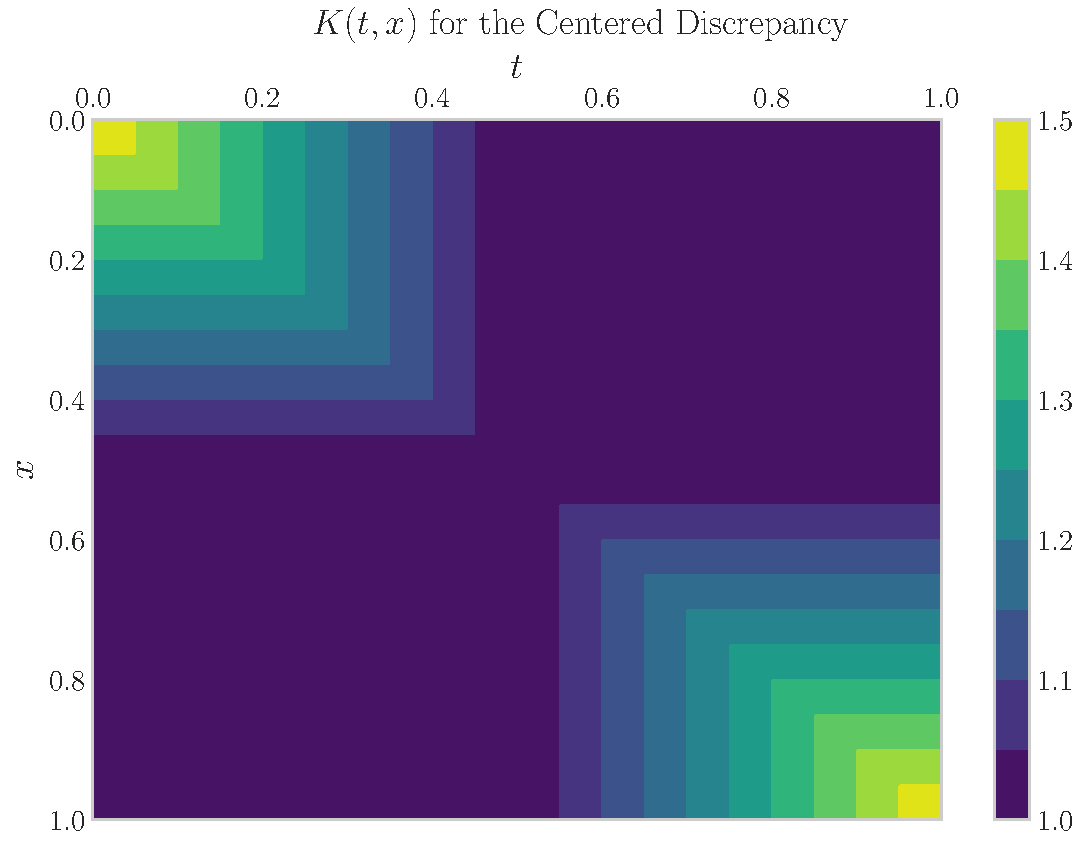
\includegraphics[width = \textwidth]{\figpath/centered_discrepancy_kernel.pdf}
	\caption{A plot of the reproducing kernel for the centered discrepancy defined in \eqref{eq:ctrkernel} for $d=1$.  Note that the vertical axis is inverted so that the plot is a picture of the ``matrix'' $\bigl( K(t,x) \bigr)_{t,x \in [0,1)]}$.  Any submatrix is positive definite by property \eqref{eq:KcondPD}. \label{fig:ctrKer}}
\end{figure}

The squared centered discrepancy is given by substituting the formula for $K$ into \eqref{eq:sqdisc}, which implies
\begin{align} \label{eq:ctrdisc}
	\nonumber
	\MoveEqLeft\text{ctr-discrepancy}^2\bigl(\{ \bsx_i\}_{i=0}^{n-1} \bigr) \\
	\nonumber
	&= \left ( \frac{13}{12} \right )^d
	- \frac 2n \sum_{i=0}^{n-1} \prod_{\ell=1}^d \left [ 1 + \frac 12 \bigl ( \lvert x_{i\ell} - 1/2 \rvert - \lvert x_{i\ell} - 1/2 \rvert^d \bigr )\right ] \\
	& \qquad \qquad \frac{1}{n^2} \sum_{i,j=0}^{n-1} \prod_{\ell = 1}^d \left[ 1 + \frac 12 \bigl ( \lvert x_{i\ell} - 1/2 \rvert + \lvert x_{j\ell} - 1/2 \rvert - \lvert x_{i\ell} - x_{j\ell} \rvert \bigr ) \right].
\end{align}
As is true for most cases, the computational cost of computing the discrepancy is $\mathcal{O}(dn^2)$ as $d$ and/or $n$ tend to infinity.

Figure \ref{fig:ctrdiscmodestd} displays the discrepancy for a Sobol' LD digital net for several modest values of $d$ and for $n =  1, 2, 4, \ldots$.  The decay rate of nearly $\calO(n^{-1})$ is observed for small $d$ and can be anticipated for a bit larger $d$.  Thus, the decay of the discrepancy mirrors the convergenc rate for LD sequences for the Kiester example in Section \ref{sec:intro} and Figure \ref{fig:keister-err}.

\begin{figure}
	\centering
	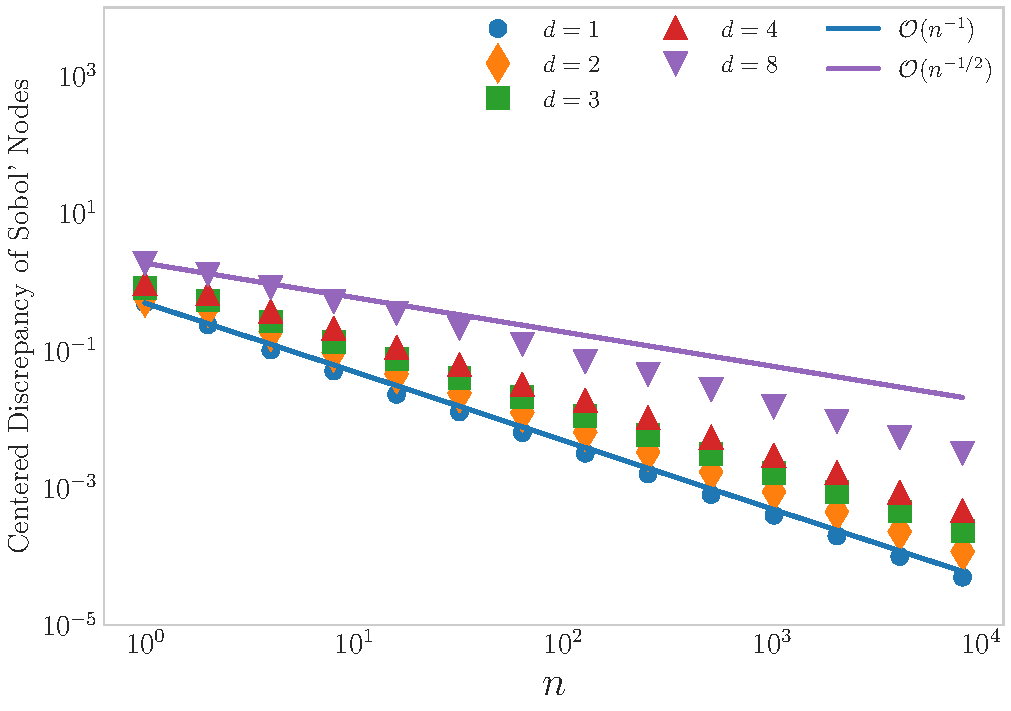
\includegraphics[width = \textwidth]{\figpath/SobolCtrDisc_n_8192_d8.pdf}
	\caption{The centered discrepancy for several modest values of $d$.  They show an asymptotic decay close to $\calO(n^{-1})$, but this rate is achieved only at higher $n$ for larger values of $d$ \label{fig:ctrdiscmodestd}}
\end{figure}

The centered discrepancy also has a geometric interpretation, as is described in \cite{Hic97a}. Other choices of kernels and their geomeetric interpretations are explained there as well.


\subsection{Coordinate weights} \label{sec:coordwts}
When the dimension, $d$, is increased, the discrepancy increases and the rate of decay with increasing sample size deteriorates, as can be seen in Figure ??.  This raises the question of whether the LD sequences lose their effectiveness for higher dimensions or whether the theory described in the pervious section does not well describe what may occur in practice.

One thing to note is that the discrepancy of the null set, which is equivalent to the norm of the linear functional $\mu(\cdot)$, is
\begin{equation}
		\text{discrepancy}\bigl(\emptyset,K \bigr)  = \sqrt{\int_{[0,1)^d \times [0,1)^d} K(\bst,\bsx) \, \mathrm{d} \bst \, \mathrm{d} \bsx},
\end{equation}
which corresponds to $(13/12)^{d/2}$ for the centered discrepancy.  This means that integration gets exponentially harder as $d$ increases.  One may scale the discrepancy of a node set by dividing it by discrepancy$(\emptyset,K)$, but this does not recover the desired nearly $\mathcal{O}(n^{-1})$ decay rate.

A better approach is to introduce coordinate weights, $\gamma_1, \ldots, \gamma_d$ into the reproducing kernel.  For the kernel defining the centered discrepancy, this means
\begin{align} \label{eq:wtctrkernel}
	K(\bst,\bsx) &= \prod_{\ell = 1}^d \biggl [ 1 + \frac {\gamma_\ell^2}2 \bigl ( \lvert t_\ell - 1/2 \rvert + \lvert x_\ell - 1/2 \rvert - \lvert t_\ell - x_\ell \rvert \bigr ) \biggr] , \\
	\langle f, g \rangle_{\calH_K}  &= \sum_{\bsell \subseteq \{1, \ldots, d\}} \prod_k \gamma_{\ell_k}^2 \langle D^{\bsell}f, D^{\bsell}g \rangle_2, \\
	\text{variation}(f)  &= \sqrt{\sum_{\bsell \subseteq \{1, \ldots, d\}} \prod_k \gamma_{\ell_k}^2 \lVert D^{\bsell}f \rVert_2^2}, \\
	\label{eq:wt-ctrdisc}
	\nonumber
	\MoveEqLeft[4]\text{wt-ctr-discrepancy}^2\bigl(\{ \bsx_i\}_{i=0}^{n-1} \bigr) \\
	\nonumber
	&= \prod_{\ell=1}^d \left ( 1 + \frac{\gamma_{\ell}^2}{12} \right )^d
	- \frac 2n \sum_{i=0}^{n-1} \prod_{\ell=1}^d \left [ 1 + \frac {\gamma_{\ell}^2}2 \bigl ( \lvert x_{i\ell} - 1/2 \rvert - \lvert x_{i\ell} - 1/2 \rvert^d \bigr )\right ] \\
	& \qquad \qquad \frac{1}{n^2} \sum_{i,j=0}^{n-1} \prod_{\ell = 1}^d \left[ 1 + \frac {\gamma_{\ell}^2}2 \bigl ( \lvert x_{i\ell} - 1/2 \rvert + \lvert x_{j\ell} - 1/2 \rvert - \lvert x_{i\ell} - x_{j\ell} \rvert \bigr ) \right].
\end{align}



\subsection{Discrepancies for Lattices and Nets} \label{sec:latticenetdis}

\subsection{Randomized Error}

\section{Stopping Criteria} \label{sec:stop}
Art

Tony

Jags

\section{Reformulating Our Problem} \label{sec:reformulate}
\subsection{Variable Transformations}
\subsection{Variation Reduction}
\subsection{Multilevel Methods}

\section{Ongoing Research} \label{sec:onging}
\section{Conclusion} \label{sec:conclusion}



\bibliographystyle{spmpsci}
\bibliography{FJH23,FJHown23}

\section*{Appendix A}
The integral $I_{\cos}(d) := \int_{0}^{\infty} \cos(r) \exp(-r^2) \, r^{d-1} \rmd r$ and its relative, the integral $I_{\sin}(d) := \int_{0}^{\infty} \sin(r) \exp(-r^2) \, r^{d-1} \rmd r$, may be evaluated iteratively for $d = 1, 2, \ldots$.  Note that using integration by parts:
\begin{align*}
I_{\cos}(d)
	&=  \left .   \cos(r) \exp(-r^2) \, \frac{r^{d}}{d}  \right \rvert_0^{\infty} \\
	& \qquad \qquad - \int_{0}^{\infty} [\cos(r) (-2r )\exp(-r^2) -\sin(r)  \exp(-r^2)] \,  \frac{r^{d}}{d} \rmd r \\
	&= \frac{2 I_{\cos}(d+2) + I_{\sin}(d+1)}{d} \\
	I_{\sin}(d) &=  \left .   \sin(r) \exp(-r^2) \, \frac{r^{d}}{d}  \right \rvert_0^{\infty} \\
	&\qquad \qquad - \int_{0}^{\infty} [\sin(r) (-2r )\exp(-r^2) + \cos(r)  \exp(-r^2)] \,  \frac{r^{d}}{d} \rmd r \\
&= \frac{2 I_{\sin}(d+2) - I_{\cos}(d+1)}{d}
\end{align*}
This implies that
\begin{align*}
	I_{\cos}(d+2) & = \frac{d I_{\cos}(d) - I_{\sin}(d+1)}{2},   \\
	I_{\sin}(d+2) &=   \frac{d I_{\sin}(d) + I_{\cos}(d+1)}{2},
\end{align*}

Need to finish and check against VS Code today

\end{document}

\iffalse
\subsection{Geometrically Motivated Discrepancies} \label{sec:geodisc}

The centered discrepancy also has a geometric explanation, as is explained in \cite{Hic97a}.  Let's explain for $d=1$, which means that we are measuring the discrepancy of points on $[0,1)$.  Consider the line segment between an arbitrary point $x$ and closesr end of the line segment.  The length of that line segment is $\lvert \ind_{[1/2,1)}(x) - x \rvert$, ,where $\ind$ is the indicator function.  The fraction of nodes that lie inside this line segment is
\begin{equation*}
	\frac 1n \sum_{i=0}^{n-1} \bigl \lvert \ind_{[1/2,1)}(x) - \ind_{[x_i,1)}(x) \bigr \rvert
\end{equation*}
A measure of discrepancy is the root mean square integral of the difference between the `fare share value'' and the actual value, i.e.,
\begin{align*}
	\text{geo-discrepancy}\bigl( \{x_i\|_{i=0}^{n-1}\}\bigr) & =
	\int_0^1 \left [ \lvert \ind_{[1/2,1)}(x) - x \rvert - \frac 1n \sum_{i=0}^{n-1} \bigl \lvert \ind_{[1/2,1)}(x) - \ind_{[x_i,1)}(x) \bigr \rvert \right ] ^2
\end{align*}

\fi


